\documentclass[a4paper]{article}

\def\npart {III}
\def\nterm {Michaelmas}
\def\nyear {2017}
\def\nlecturer {C. Warnick}
\def\ncourse {Analysis of Partial Differential Equations}
\def\ncoursehead {Analysis of PDEs}

% example classes : https://tinyurl.com/partiiiPDE

% Imports
\ifx \nextra \undefined
  \usepackage[pdftex,
    hidelinks,
    pdfauthor={Dexter Chua},
    pdfsubject={Cambridge Maths Notes: Part \npart\ - \ncourse},
    pdftitle={Part \npart\ - \ncourse},
  pdfkeywords={Cambridge Mathematics Maths Math \npart\ \nterm\ \nyear\ \ncourse}]{hyperref}
  \title{Part \npart\ - \ncourse}
\else
  \usepackage[pdftex,
    hidelinks,
    pdfauthor={Dexter Chua},
    pdfsubject={Cambridge Maths Notes: Part \npart\ - \ncourse\ (\nextra)},
    pdftitle={Part \npart\ - \ncourse\ (\nextra)},
  pdfkeywords={Cambridge Mathematics Maths Math \npart\ \nterm\ \nyear\ \ncourse\ \nextra}]{hyperref}

  \title{Part \npart\ - \ncourse \\ {\Large \nextra}}
\fi

\author{Lectured by \nlecturer \\\small Notes taken by Dexter Chua}
\date{\nterm\ \nyear}

\usepackage{alltt}
\usepackage{amsfonts}
\usepackage{amsmath}
\usepackage{amssymb}
\usepackage{amsthm}
\usepackage{booktabs}
\usepackage{caption}
\usepackage{enumitem}
\usepackage{fancyhdr}
\usepackage{graphicx}
\usepackage{mathtools}
\usepackage{microtype}
\usepackage{multirow}
\usepackage{pdflscape}
\usepackage{pgfplots}
\usepackage{siunitx}
\usepackage{tabularx}
\usepackage{tikz}
\usepackage{tkz-euclide}
\usepackage[normalem]{ulem}
\usepackage[all]{xy}

\pgfplotsset{compat=1.12}

\pagestyle{fancyplain}
\lhead{\emph{\nouppercase{\leftmark}}}
\ifx \nextra \undefined
  \rhead{
    \ifnum\thepage=1
    \else
      \npart\ \ncourse
    \fi}
\else
  \rhead{
    \ifnum\thepage=1
    \else
      \npart\ \ncourse\ (\nextra)
    \fi}
\fi
\usetikzlibrary{arrows}
\usetikzlibrary{decorations.markings}
\usetikzlibrary{decorations.pathmorphing}
\usetikzlibrary{positioning}
\usetikzlibrary{fadings}
\usetikzlibrary{intersections}
\usetikzlibrary{cd}

\newcommand*{\Cdot}{\raisebox{-0.25ex}{\scalebox{1.5}{$\cdot$}}}
\newcommand {\pd}[2][ ]{
  \ifx #1 { }
    \frac{\partial}{\partial #2}
  \else
    \frac{\partial^{#1}}{\partial #2^{#1}}
  \fi
}

% Theorems
\theoremstyle{definition}
\newtheorem*{aim}{Aim}
\newtheorem*{axiom}{Axiom}
\newtheorem*{claim}{Claim}
\newtheorem*{cor}{Corollary}
\newtheorem*{defi}{Definition}
\newtheorem*{eg}{Example}
\newtheorem*{fact}{Fact}
\newtheorem*{law}{Law}
\newtheorem*{lemma}{Lemma}
\newtheorem*{notation}{Notation}
\newtheorem*{prop}{Proposition}
\newtheorem*{thm}{Theorem}

\renewcommand{\labelitemi}{--}
\renewcommand{\labelitemii}{$\circ$}
\renewcommand{\labelenumi}{(\roman{*})}

\let\stdsection\section
\renewcommand\section{\newpage\stdsection}

% Strike through
\def\st{\bgroup \ULdepth=-.55ex \ULset}

% Maths symbols
\newcommand{\bra}{\langle}
\newcommand{\ket}{\rangle}

\newcommand{\N}{\mathbb{N}}
\newcommand{\Z}{\mathbb{Z}}
\newcommand{\Q}{\mathbb{Q}}
\renewcommand{\H}{\mathbb{H}}
\newcommand{\R}{\mathbb{R}}
\newcommand{\C}{\mathbb{C}}
\newcommand{\Prob}{\mathbb{P}}
\renewcommand{\P}{\mathbb{P}}
\newcommand{\E}{\mathbb{E}}
\newcommand{\F}{\mathbb{F}}
\newcommand{\cU}{\mathcal{U}}
\newcommand{\RP}{\mathbb{RP}}
\newcommand{\CP}{\mathbb{CP}}

\newcommand{\ph}{\,\cdot\,}

\DeclareMathOperator{\sech}{sech}
\DeclareMathOperator{\cosech}{cosech}
\DeclareMathOperator{\cosec}{cosec}

\DeclareMathOperator{\covol}{covol}
\DeclareMathOperator{\vol}{vol}

\let\Im\relax
\let\Re\relax
\DeclareMathOperator{\Im}{Im}
\DeclareMathOperator{\Re}{Re}
\DeclareMathOperator{\im}{im}
\DeclareMathOperator{\image}{image}
\DeclareMathOperator{\Ann}{Ann}

\DeclareMathOperator*{\res}{res}
\DeclareMathOperator{\Res}{Res}
\DeclareMathOperator{\Ind}{Ind}

\DeclareMathOperator{\tr}{tr}
\DeclareMathOperator{\diag}{diag}
\DeclareMathOperator{\rank}{rank}
\DeclareMathOperator{\card}{card}
\DeclareMathOperator{\spn}{span}
\DeclareMathOperator{\adj}{adj}

\DeclareMathOperator{\erf}{erf}
\DeclareMathOperator{\erfc}{erfc}

\DeclareMathOperator{\ord}{ord}
\DeclareMathOperator{\Sym}{Sym}

\DeclareMathOperator{\sgn}{sgn}
\DeclareMathOperator{\orb}{orb}
\DeclareMathOperator{\stab}{stab}
\DeclareMathOperator{\ccl}{ccl}

\DeclareMathOperator{\lcm}{lcm}
\DeclareMathOperator{\hcf}{hcf}

\DeclareMathOperator{\Int}{Int}
\DeclareMathOperator{\id}{id}

\DeclareMathOperator{\betaD}{beta}
\DeclareMathOperator{\gammaD}{gamma}
\DeclareMathOperator{\Poisson}{Poisson}
\DeclareMathOperator{\binomial}{binomial}
\DeclareMathOperator{\multinomial}{multinomial}
\DeclareMathOperator{\Bernoulli}{Bernoulli}
\DeclareMathOperator{\like}{like}

\DeclareMathOperator{\var}{var}
\DeclareMathOperator{\cov}{cov}
\DeclareMathOperator{\bias}{bias}
\DeclareMathOperator{\mse}{mse}
\DeclareMathOperator{\corr}{corr}

\DeclareMathOperator{\otp}{otp}
\DeclareMathOperator{\dom}{dom}

\DeclareMathOperator{\Root}{Root}
\DeclareMathOperator{\supp}{supp}
\DeclareMathOperator{\rel}{rel}
\DeclareMathOperator{\Hom}{Hom}
\DeclareMathOperator{\Aut}{Aut}
\DeclareMathOperator{\Gal}{Gal}
\DeclareMathOperator{\Mat}{Mat}
\DeclareMathOperator{\End}{End}
\DeclareMathOperator{\Char}{char}
\DeclareMathOperator{\ev}{ev}
\DeclareMathOperator{\St}{St}
\DeclareMathOperator{\Lk}{Lk}
\DeclareMathOperator{\disc}{disc}
\DeclareMathOperator{\Isom}{Isom}
\DeclareMathOperator{\length}{length}
\DeclareMathOperator{\energy}{energy}
\DeclareMathOperator{\area}{area}
\DeclareMathOperator{\Syl}{Syl}
\DeclareMathOperator{\cl}{cl}
\DeclareMathOperator{\fix}{fix}

\newcommand{\GL}{\mathrm{GL}}
\newcommand{\SL}{\mathrm{SL}}
\newcommand{\PGL}{\mathrm{PGL}}
\newcommand{\PSL}{\mathrm{PSL}}
\newcommand{\PSU}{\mathrm{PSU}}
\newcommand{\Or}{\mathrm{O}}
\newcommand{\SO}{\mathrm{SO}}
\newcommand{\U}{\mathrm{U}}
\newcommand{\SU}{\mathrm{SU}}

\renewcommand{\d}{\mathrm{d}}
\newcommand{\D}{\mathrm{D}}

\tikzset{->/.style = {decoration={markings,
                                  mark=at position 1 with {\arrow[scale=2]{latex'}}},
                      postaction={decorate}}}
\tikzset{<-/.style = {decoration={markings,
                                  mark=at position 0 with {\arrowreversed[scale=2]{latex'}}},
                      postaction={decorate}}}
\tikzset{<->/.style = {decoration={markings,
                                   mark=at position 0 with {\arrowreversed[scale=2]{latex'}},
                                   mark=at position 1 with {\arrow[scale=2]{latex'}}},
                       postaction={decorate}}}
\tikzset{->-/.style = {decoration={markings,
                                   mark=at position #1 with {\arrow[scale=2]{latex'}}},
                       postaction={decorate}}}
\tikzset{-<-/.style = {decoration={markings,
                                   mark=at position #1 with {\arrowreversed[scale=2]{latex'}}},
                       postaction={decorate}}}

\tikzset{circ/.style = {fill, circle, inner sep = 0, minimum size = 3}}
\tikzset{mstate/.style={circle, draw, blue, text=black, minimum width=0.7cm}}

\definecolor{mblue}{rgb}{0.2, 0.3, 0.8}
\definecolor{morange}{rgb}{1, 0.5, 0}
\definecolor{mgreen}{rgb}{0.1, 0.4, 0.2}
\definecolor{mred}{rgb}{0.5, 0, 0}

\def\drawcirculararc(#1,#2)(#3,#4)(#5,#6){%
    \pgfmathsetmacro\cA{(#1*#1+#2*#2-#3*#3-#4*#4)/2}%
    \pgfmathsetmacro\cB{(#1*#1+#2*#2-#5*#5-#6*#6)/2}%
    \pgfmathsetmacro\cy{(\cB*(#1-#3)-\cA*(#1-#5))/%
                        ((#2-#6)*(#1-#3)-(#2-#4)*(#1-#5))}%
    \pgfmathsetmacro\cx{(\cA-\cy*(#2-#4))/(#1-#3)}%
    \pgfmathsetmacro\cr{sqrt((#1-\cx)*(#1-\cx)+(#2-\cy)*(#2-\cy))}%
    \pgfmathsetmacro\cA{atan2(#2-\cy,#1-\cx)}%
    \pgfmathsetmacro\cB{atan2(#6-\cy,#5-\cx)}%
    \pgfmathparse{\cB<\cA}%
    \ifnum\pgfmathresult=1
        \pgfmathsetmacro\cB{\cB+360}%
    \fi
    \draw (#1,#2) arc (\cA:\cB:\cr);%
}
\newcommand\getCoord[3]{\newdimen{#1}\newdimen{#2}\pgfextractx{#1}{\pgfpointanchor{#3}{center}}\pgfextracty{#2}{\pgfpointanchor{#3}{center}}}

\def\Xint#1{\mathchoice
   {\XXint\displaystyle\textstyle{#1}}%
   {\XXint\textstyle\scriptstyle{#1}}%
   {\XXint\scriptstyle\scriptscriptstyle{#1}}%
   {\XXint\scriptscriptstyle\scriptscriptstyle{#1}}%
   \!\int}
\def\XXint#1#2#3{{\setbox0=\hbox{$#1{#2#3}{\int}$}
     \vcenter{\hbox{$#2#3$}}\kern-.5\wd0}}
\def\ddashint{\Xint=}
\def\dashint{\Xint-}


\begin{document}
\maketitle
{\small
\setlength{\parindent}{0em}
\setlength{\parskip}{1em}

This course serves as an introduction to the mathematical study of Partial Differential Equations (PDEs). The theory of PDEs is nowadays a huge area of active research, and it goes back to the very birth of mathematical analysis in the 18th and 19th centuries. The subject lies at the crossroads of physics and many areas of pure and applied mathematics.

The course will mostly focus on four prototype linear equations: Laplace's equation, the heat equation, the wave equation and Schr\"odinger's equation. Emphasis will be given to modern functional analytic techniques, relying on a priori estimates, rather than explicit solutions, although the interaction with classical methods (such as the fundamental solution and Fourier representation) will be discussed. The following basic unifying concepts will be studied: well-posedness, energy estimates, elliptic regularity, characteristics, propagation of singularities, group velocity, and the maximum principle. Some non-linear equations may also be discussed. The course will end with a discussion of major open problems in PDEs.

\subsubsection*{Pre-requisites}
There are no specific pre-requisites beyond a standard undergraduate analysis background, in particular a familiarity with measure theory and integration. The course will be mostly self-contained and can be used as a first introductory course in PDEs for students wishing to continue with some specialised PDE Part III courses in the Lent and Easter terms.
}
\tableofcontents

\section{Introduction}
This is a course on partial differential equations. So it might be wise to define what a partial differential equation is.

\begin{defi}[Partial differential equation]
  Suppose $U \subseteq \R^n$ is open. A \term{partial differential equation} (\term{PDE}) of \emph{order}\index{order of PDE}\index{PDE!order} $k$ is a relation of the form
  \[
    F(x, U(x), \D U(x), \ldots, \D^k u(x)) = 0,\tag{$*$}
  \]
  where $F: U \times \R \times \R^n \times \R^{n^2} \times \cdots \times \R^{n^k} \to \R$ is a given function, and $u: U \to \R$ is the ``unknown''.
\end{defi}

\begin{defi}[Classical solution]
  We say $u \in C^k(U)$ is a \term{classical solution} of a PDE if in fact the PDE is identically satisfied on $U$ when $u, \D u, \ldots, \D^k u$ are substituted in.
\end{defi}

More generally, we can allow $u$ and $F$ to take values in a vector space. In this case, we say it is a \term{system of PDEs}\index{PDE!system}\index{partial differential equation!system}.

We can now entertain ourselves by writing out a large list of PDEs that are naturally found in physics and mathematics.
\begin{eg}[Transport equation]\index{transport equation}
  Suppose $v: \R^4 \times \R \to \R^3$ and $j: \R^4 \to \R$ are given. The \emph{transport equation} is
  \[
    \frac{\partial u}{\partial t}(x, t) + v(x, t, u(x, t)) \cdot \D_x u(x, t) = f(x, t)
  \]
  where we think of $x \in \R^3$ and $t \in \R$. This describes the evolution of the density $u$ of some chemical being advected by a flow $v$ and produced at a rate $f$.

  We see that this is a PDE of order $1$, and a relatively straightforward solution method exists, namely the \term{method of characteristics}.
\end{eg}

\begin{eg}[Laplace's and Poissson's equations]\index{Laplace's equation}\index{Poisson's equation}
  Taking $u: \R^n \to \R$, Laplace's equation is
  \[
    \Delta u(x) = \sum_{i = 1}^n \frac{\partial^2 u}{\partial x_i \partial x_i} (x) = 0.
  \]
  This describes, for example, the electrostatic potential in vacuum and the static distribution of heat inside a uniform solid body. it also has applications to steady flows in 2d fluids.

  There is an inhomogeneous version of this:
  \[
    \Delta u(x) = f(x),
  \]
  where $f: \R^n \to \R$ is a fixed function. This is known as \emph{Poisson's equation}, and describes, for example, the electrostatic field due to a charge distribution, and the gravitational field in Newtonian gravity.
\end{eg}

\begin{eg}[Heat/diffusion equation]\index{heat equation}\index{diffusion equation}
  This is given by
  \[
    \frac{\partial u}{\partial t} = \Delta u,
  \]
  where $u: \R^n \times \R \to \R$ is now a function of space and time. This describes the evolution of temperature inside a uniform body, or equivalently the diffusion of some chemical (where $u$ is the density).
\end{eg}

\begin{eg}[Wave equation]\index{wave equation}
  The wave equation is given by
  \[
    \frac{\partial^2 u}{\partial t^2} = \Delta u,
  \]
  where $u: \R^n \times \R \to \R$ is again a function of space and time. This describes oscillations of
  \begin{itemize}
    \item strings ($n = 1$)
    \item membrane/drum ($n = 2$)
    \item air density in a sound wave ($n = 3$)
  \end{itemize}
\end{eg}

\begin{eg}[Schr\"odinger's equation]\index{Schr\"odinger's equation}
  Let $u: \R^n \times \R \to \C \cong \R^2$. Up to choices of units and convention, the \emph{Schr\"odinger's equation} is
  \[
    i\frac{\partial u}{\partial t} + \Delta u - Vu = 0.
  \]
  Here $u$ is the wavefunction of a particle moving in a potential $V: \R^n \to \R$.
\end{eg}

\begin{eg}[Maxwell's equations]\index{Maxwell's equation}
  The unknowns here are $\mathbf{E}, \mathbf{B}: \R^3 \times \R \to \R^3$. They satisfy \emph{Maxwell's equations}
  \begin{align*}
    \nabla \cdot \mathbf{E} &= 0 & \nabla \cdot \mathbf{B} &= 0\\
    \nabla \times \mathbf{E} + \frac{\partial \mathbf{B}}{\partial t} &= 0 & \nabla \times \mathbf{B} - \frac{\partial \mathbf{E}}{\partial t} &= \mathbf{J},
  \end{align*}
  where $\rho$ is the electric charge density, $\mathbf{J}$ is the electric current, $\mathbf{E}$ is the electric field and $\mathbf{B}$ is the magnetic field.

  This is a system of 6 equations and 6 unknowns.
\end{eg}

\begin{eg}[Einstein's equations]\index{Einstein's equations}
  The \emph{Einstein's equation} in vacuum are
  \[
    R_{\mu\nu}[g] = 0,
  \]
  where $g$ is a Lorentzian metric (encoding the gravitational field), and $R_{\mu\nu}[g]$ is the Ricci curvature of $g$.

  Since we haven't said what $g$ and $R_{\mu\nu}$ are, it is not clear that this is a partial differential equation, but it is.
\end{eg}

\begin{eg}[Minimal surface equation]\index{minimal surface equation}
  The \emph{minimal surface equation is}
  \[
    \mathrm{Div}\left(\frac{\D u}{\sqrt{1 + |\D u|^2}}\right) = 0,
  \]
  where $u: \R^n \to \R$ is some function. This is the condition that the graph of $u$, $\{(x, u(x)\}\subseteq \R^n \times \R$, is locally an extremizer of area.
\end{eg}

\begin{eg}[Ricci flow]\index{Ricci flow}
  Let $g$ be a Riemannian metric on some manifold. The \emph{Ricci flow} is a PDE that evolves this metric:
  \[
    \frac{\partial g_{ij}}{\partial t} = R_{ij}[g],
  \]
  where $R_{ij}$ is again the Ricci curvature.

  The most famous application is in proving the Poincar\'e conjecture, which is a topological conjecture about $3$-manifolds.
\end{eg}

So what do want to know about PDEs? The first thing to note is that these PDEs exhibit a wide variety of behaviours. For example, waves behave very differently from the evolution of temperature. This means it is unlikely that we can say anything about PDEs as a whole, since everything we say must be true for both the heat equation and the wave equation. We must restrict to some particular classes of PDEs to say something useful.

\subsection{Data and well-posedness}
In all the examples, we need some additional information to even hope for a unique solution. For example, in the case of Laplace's equation, we might need to know the boundary values of $u$; For the heat equation, we need to know the initial temperature distribution. We broadly refer to these information as the \term{data}. An important part of studying PDE is to understand what data we need for a certain PDE problem. Roughly speaking, we want enough data so that we can solve the problem, and not too much data that there is no solution.

A guiding principle in this regard is \emph{well-posedness}.
\begin{defi}[Well-posed problem]\index{well-posed problem}
  We say a PDE problem (equation plus data) is \term{well-posed} if
  \begin{enumerate}
    \item A solution exists;
    \item The solution is unique; and
    \item The solution depends continuously on the data.
  \end{enumerate}
\end{defi}
We should make this more precise. To say whether a solution exists, we need to first specify a function space, and ask if there is a solution in that function space. The same goes for the uniqueness problem. To ask whether the solution depends continuously, we must put the solution and data in appropriate function spaces that come with a topology.

There is a certain freedom for us to choose which function space we are looking at, and there is no god-given choice. There is some tension between our requirements --- if we want our solution to exist, it is better to work with a larger function space; if we want it to be unique, we want it to be smaller. The details of whether a problem is well-posed can depend on the choice of function space.

In this course, the natural numbers start at $0$.
\begin{notation}[Multi-index/Schwartz notation]\index{multi-index notation}\index{Schwartz notation}
  We say an element $\alpha \in \N^n$ is a \emph{multi-index}. Writing $\alpha = (\alpha_1, \ldots, \alpha_n)$. We write
  \[
    |\alpha| = \alpha_1 + \alpha_2 + \cdots + \alpha_n.
  \]
  Also, we have
  \[
    \D^\alpha f(x) = \frac{\partial^{|\alpha|}f}{\partial x_1^{\alpha_1} \partial x_2^{\alpha_2} \cdots \partial x_n^{\alpha_n}}.
  \]
  If $x = (x_1, \ldots, x_n) \in \R^n$, then
  \[
    x^\alpha = x_1^{\alpha_1} x_2^{\alpha_2} \cdots x_n^{\alpha_n}.
  \]
  We also write
  \[
    \alpha! = \alpha_1! \alpha_2! \cdots \alpha_n!.
  \]
\end{notation}

We now try to crudely classify the PDEs we have written down. Recall that our PDEs take the general form
\[
  F(x, U(x), \D U(x), \ldots, \D^k u(x)) = 0.
\]

\begin{defi}[Linear PDE]\index{linear PDE}\index{PDE!linear}
  We say a PDE is \emph{linear} if $F$ is a linear function of $u$ and its derivatives. In this case, we can re-write it as
  \[
    \sum_{|\alpha| \leq k} a_\alpha(x) \D^\alpha u = 0.
  \]
\end{defi}

\begin{defi}[Semi-linear PDE]\index{semi-linear PDE}\index{PDE!semi-linear}
  We say a PDE is \emph{semi-linear} if it is of the form
  \[
    \sum_{|\alpha| = k} a_\alpha(x) \D^\alpha u(x) + a_0[x, u, \D u, \ldots, \D^{k - 1} u] = 0.
  \]
  In other words, the terms involving the highest order derivatives are linear.
\end{defi}
Generalizing further, we have
\begin{defi}[Quasi-linear PDE]\index{quasi-linear PDE}\index{PDE!quasi-linear}
  We say a PDE is \emph{quasi-linear} if it is of the form
  \[
    \sum_{|\alpha| = k} a_\alpha [x, u, \D u, \ldots, \D^{k - 1} u] \D^\alpha u(x) + a_0[x, u, \ldots, \D^{k - 1} u] = 0.
  \]
\end{defi}
So the highest order derivative still appears linearly, but the coefficients can depend on lower-order derivatives of $u$.

Finally, we have
\begin{defi}[Fully non-linear PDE]\index{fully non-linear PDE}\index{PDE!fully non-linear}
  A PDE is \emph{fully non-linear} if it is not quasi-linear.
\end{defi}

\begin{eg}
  Laplace's equation $\Delta u = 0$ is linear.
\end{eg}

\begin{eg}
  The equation $u_{xx} + u_{yy} = u_x^2$ is semi-linear.
\end{eg}

\begin{eg}
  The equation $uu_{xx} u_{yy} = u_x^2$ is quasi-linear.
\end{eg}

\begin{eg}
  The equation $u_{xx} u_{yy} - u_{xy}^2 = 0$ is fully non-linear.
\end{eg}

\section{The Cauchy--Kovalevskaya theorem}

\subsection{The Cauchy--Kovalevskaya theorem}
Before we begin talking about PDEs, let's recall what we already know about ODEs. Fix some $U \subseteq \R^n$ an open subset, and assume $f: U \to \R^n$ is given. Consider the ODE
\[
  \dot{u}(t) = f(u(t)).
\]
This is an \term{autonomous ODE}\index{ODE!autonomous} because there is no explicit $t$ dependence on the right. This assumption is usually harmless, as we can just increment $n$ and use the new variable to keep track of $t$. Here $u: (a, b) \to U$ is the unknown, where $a < 0 < b$.

The \term{Cauchy problem} for this equation is to find a solution to the ODE satisfying $u(0) = u_0 \in U$ for any $u_0$.

The Picard--Lindel\"of theorem says we can always do so under some mild conditions.
\begin{thm}[Picard--Lindel\"of theorem]\index{Picard--Lindelof theorem}
  Suppose that there exists $r, K > 0$ such that $B_r(u_0) \subseteq U$, and
  \[
    \|f(x) - f(y)\| \leq K \|x - u\|
  \]
  for all $x, y \in B_r(u_0)$. Then there exists an $\varepsilon > 0$ depending on $K, r$ and a unique $C^1$ function $u: (-\varepsilon, \varepsilon) \to U$ solving the Cauchy problem.
\end{thm}

It is instructive to give a quick proof sketch of the result.

\begin{proof}[Proof sketch]
  If $u$ is a solution, then by the fundamental theorem of calculus, we have
  \[
    u(t) = u_0 + \int_0^t f(u(s))\;\d s.
  \]
  Conversely, if $u$ is a $C^0$ solution to this integral equation, then it solves the ODE. Crucially, this only requires $u$ to be $C^0$. Indeed, if $u$ is $C^0$ and satisfies the integral equation, then $u$ is automatically $C^1$. So we can work in a larger function space when we seek for $u$.

  Thus, we have reformulated our initial problem into an integral equation. In particular, we reformulated it in a way that assumes less about the function. In the case of PDEs, this is what is known as a \term{weak formulation}.

  Returning to the proof, we have reformulated our problem as looking for a fixed point of the map
  \[
    B: w \mapsto u_0+ \int_0^t f(w(s))\;\d s
  \]
  acting on
  \[
    \mathcal{C} = \{w: [-\varepsilon, \varepsilon] \to \overline{B_{r/2}(u_0)} : w\text{ is continuous}\}.
  \]
  This is a complete metric space when we equip it with the supremum norm (in fact, it is a closed ball in a Banach space).

  We then show that for $\varepsilon$ small enough, this map $B: \mathcal{C} \to \mathcal{C}$ is a contraction map. There are two parts --- to show that it actually lands in $\mathcal{C}$, and that it is a contraction. If we managed to show these, then by the contraction mapping theorem, there is a unique fixed point, and we are done.
\end{proof}

The idea of formulating our problem as a fixed point problem is a powerful technique that allows us to understand many PDEs, especially non-linear ones. This theorem tells us that a unique $C^1$ solution exists locally. It is not reasonable to believe it can exist globally, as we might run out of $U$ in finite time. However, if $f$ is better behaved, we might expect $u$ to be more regular, and indeed this is the case. We shall not go into the details.

How can we actually use the theorem in practice? Can we actually obtain a solution from this? Recall that to prove the contraction mapping theorem, what we do is that we arbitrarily pick a point in $\mathcal{C}$, keep applying $\mathcal{B}$, and by the contraction, we must approach the fixed point. This gives us a way to construct an approximation to the ODE.

However, if we were a physicist, we would have done things differently. Suppose $f \in C^\infty$. We can then attempt to construct a Taylor series of the solution near the origin. First we note that for any solution $u$, we must have
\[
   u(0) = u_0,\quad \dot{u}(0) = f(u_0).
\]
Assuming $u$ is in fact a smooth solution, we can differentiate the ODE and obtain
\[
  \ddot{u}(t) = \frac{\d}{\d t} \dot{u}(t) = \frac{\d}{\d t} f(u(t)) = \D f(u(t)) \dot{u}(t) \equiv f_2(u(t), \dot{u}(t)).
\]
At the origin, we already know what $u$ and $\dot{u}$. We can proceed iteratively to determine
\[
  u^{(k)}(t) = f_k (u, \dot{u}, \ldots, u^{(k - 1)}).
\]
So in particular, we can in principle determine $u_k \equiv u^{(k)} = 0$. At least formally, we can write
\[
  u(t) = \sum_{k = 0}^\infty u_k \frac{t^k}{k!}.
\]
If we were physicists, we would say we are done. But being honest mathematicians, in order to claim that we have a genuine solution, we need to at least show that this converges. Under suitable circumstances, this is given by the Cauchy--Kovalevskaya theorem.

\begin{thm}[Cauchy--Kovalevskaya for ODEs]\index{Cauchy--Kovalevskaya theorem!for ODEs}\index{ODE!Cauchy--Kovalevskaya theorem}
  The series
  \[
    u(t) = \sum_{k = 0}^\infty u_k \frac{t^k}{k!}.
  \]
  converges to the Picard--Lindel\"of solution of the Cauchy problem if $f$ is real analytic in a neighbourhood of $u_0$.
\end{thm}

Recall that being real analytic means being equal to its Taylor series:
\begin{defi}[Real analytic]\index{real analytic}\index{analytic!real}
  Let $U \subseteq \R^n$ be open, and suppose $f: U \to \R$. We say $f$ is \emph{real analytic} near $x_0 \in U$ if there exists $r > 0$ and constants $f_\alpha \in \R$ for each multi-index $\alpha$ such that
  \[
    f(x) = \sum_\alpha f_\alpha (x - x_0)^\alpha
  \]
  for $|x - x_0| < r$.
\end{defi}

Note that if $f$ is real analytic near $x_0$, then it is in fact $C^\infty$ in the corresponding neighbourhood. Furthermore, the constants $f_\alpha$ are given by
\[
  f_\alpha = \frac{1}{\alpha!} \D^\alpha f(x_0).
\]
In other words, $f$ equals its Taylor expansion. Of course, by translation, we can usually assume $x_0 = 0$.

\begin{eg}
  If $r > 0$, set
  \[
    f(x) = \frac{r}{r - (x_1 + x_2 + \cdots + x_n)}
  \]
  for $|x| < \frac{r}{\sqrt{n}}$. Then this is real analytic, since we have
  \[
    f(x) = \frac{1}{1 - (x_1 + \cdots + x_n)/r} = \sum_{k = 0}^\infty \left(\frac{x_1 + \cdots + x_n}{r}\right)^k.
  \]
  We can then expand out each term to see that this is given by a power series. Explicitly, it is given by
  \[
    f(x) = \sum_\alpha \frac{1}{r^{|\alpha|}}\binom{|\alpha|}{\alpha} x^\alpha,
  \]
  where
  \[
    \binom{|\alpha|}{\alpha} = \frac{|\alpha|!}{\alpha!}.
  \]
  One sees that this series is absolutely convergent for $|x| < \frac{r}{\sqrt{n}}$.
\end{eg}
Recall that in single-variable analysis, essentially the only way we have to show that a series converges is by comparison to the geometric series. Here with multiple variables, our only way to show that a power series converges is by comparing it to this $f$.

\begin{defi}[Majorant]\index{majorant}\index{majorize}
  Let
  \[
    f = \sum_\alpha f_\alpha x^\alpha,\quad g = \sum_\alpha g_\alpha x^\alpha
  \]
  be formal power series. We say $g$ majorizes $f$ (or $g$ is a majorant of $f$), written $g \gg f$, if $g_\alpha \geq |f_\alpha|$ for all multi-indices $\alpha$.

  If $f$ and $A$ are vector-valued, then this means $g^i \gg f^i$ for all indices $i$.
\end{defi}

\begin{lemma}\leavevmode
  \begin{enumerate}
    \item If $g \gg f$ and $g$ converges for $|x| < r$, then $f$ converges for $|x| < r$.
    \item If $f(x) = \sum_\alpha f_\alpha x^\alpha$ converges for $x < r$ and $0 < s\sqrt{n} < r$, then $f$ has a majorant which converges on $|x| < s$. % check
  \end{enumerate}
\end{lemma}

\begin{proof}\leavevmode
  \begin{enumerate}
    \item Given $x$, define $\tilde{x} = (|x_1|, |x_2|, \ldots, |x_n|)$. We then note that
      \[
        \sum_\alpha |f_\alpha x^\alpha| = \sum_\alpha |f_\alpha| \tilde{x}^\alpha \leq \sum_\alpha g_\alpha \tilde{x}^\alpha = g(\tilde{x}).
      \]
      Since $|\tilde{x}| = |x| < r$, we know $g$ converges at $\tilde{x}$.
    \item Let $0 < s\sqrt{n} < r$ and set $y = s(1, 1, \ldots, 1)$. Then we have
      \[
        |y| = s \sqrt{n} < r.
      \]
      So by assumption, we know
      \[
        \sum_\alpha f_\alpha y^\alpha
      \]
      converges. A convergent series has bounded terms, so there exists $C$ such that
      \[
        |f_\alpha y^\alpha| \leq C
      \]
      for all $\alpha$. But $y^\alpha = s^{|\alpha|}$. So we know
      \[
        |f_\alpha| \leq \frac{C}{s^{|\alpha|}} \leq \frac{C}{s^{|\alpha|}} \frac{|\alpha|!}{\alpha!}.
      \]
      But then if we set
      \[
        g(x) = \frac{Cs}{s - (x_1 + \cdots + x_n)} = C \sum_\alpha \frac{|\alpha|!}{s^{|\alpha|}\alpha!} x^\alpha,
      \]
      we are done, since this converges for $|x| < \frac{s}{\sqrt{n}}$.
  \end{enumerate}
\end{proof}

With this lemma in mind, we can now prove the Cauchy--Kovalevskaya theorem for first-order PDEs. This concerns a class of problems similar to the Cauchy problem for ODEs. We first set up our notation.

We shall consider functions $\mathbf{u}: \R^n \to \R^m$. Writing $\mathbf{x} = (x^1, \ldots, x^n) \in \R^n$, we will consider the last variable $x^n$ as being the ``time variable'', and the others as being space. However, for notational convenience, we will not write it as $t$. We will adopt the shorthand $x' = (x^1, \ldots, x^{n - 1})$, so that $\mathbf{x} = (x', x^n)$.

Suppose we are given two real analytic functions
\begin{align*}
  B: \R^m \times \R^{n - 1} &\to \Mat_{m \times m}(\R)\\
  \mathbf{c}: \R^m \times \R^{n - 1} &\to \R^m.
\end{align*}
We seek a solution to the PDE
\[
  \mathbf{u}_{x^n} = \sum_{j = 1}^{n - 1}B(\mathbf{u}, x') \mathbf{u}_{x_j} + \mathbf{c}(\mathbf{u}, x')
\]
subject to $\mathbf{u} = 0$ when $x^n = 0$. We shall not require a solution on all of $\R^n$, but only on an open neighbourhood of the origin. Consequently, we will allow for $B$ and $\mathbf{c}$ to not be everywhere defined, but merely convergent on some neighbourhood of the identity.

Note that we assumed $B$ and $\mathbf{c}$ do not depend on $x^n$, but this is not a restriction, since we can always introduce a new variable $u^{m + 1} = x^n$, and enlarge the target space.

\begin{thm}[Cauchy--Kovalevskaya theorem]\index{Cauchy--Kovalevskaya theorem!for PDEs}\index{PDE!Cauchy--Kovalevskaya theorem}
  Given the above assumptions, there exists a real analytic function $\mathbf{u} = \sum_\alpha \mathbf{u}_\alpha x^\alpha$ solving the PDE in a neighbourhood of the origin. Moreover, it is unique among real analytic functions.
\end{thm}

The uniqueness part of the proof is not difficult. If we write out $\mathbf{u}$, $B$ and $\mathbf{c}$ in power series and plug them into the PDE, we can then simply collect terms and come up with an expression for what $\mathbf{u}$ must be. This is the content of the following lemma:

\begin{lemma}
  For $k = 1, \ldots, m$ and $\alpha$ a multi-index in $\N^n$, there exists a polynomial $q_\alpha^k$ in the power series coefficients of $B$ and $\mathbf{c}$ such that any analytic solution to the PDE must be given by
  \[
    \mathbf{u} = \sum_{\alpha} \mathbf{q}_\alpha(B, \mathbf{c}) x^\alpha,
  \]
  where $\mathbf{q}_\alpha$ is the vector with entries $q_\alpha^k$.

  Moreover, all coefficients of $q_\alpha$ are non-negative.
\end{lemma}
Note that despite our notation, $\mathbf{q}$ is not a function of $B$ and $\mathbf{c}$ (which are themselves functions of $\mathbf{u}$ and $x$). It is a function of the coefficients in the power series expansion of $B$ and $\mathbf{c}$, which are some fixed constants.

This lemma proves uniqueness. To prove existence, we must show that this converges in a neighbourhood of the origin, and for this purpose, the fact that the coefficients of $q_\alpha$ are non-negative is crucial. After we have established this, we will use the comparison test to reduce the theorem to the case of a single, particular PDE, which we can solve by hand.

\begin{proof}
%  By assumption, we can expand $B$ and $\mathbf{c}$ as power series:
%  \begin{align*}
%    B_j(\mathbf{z}, x') &= \sum_{\gamma, \delta} B_{j, \gamma, \delta} z^\gamma x^\delta\\
%    \mathbf{c}(\mathbf{z}, x') &= \sum_{\gamma, \delta} \mathbf{c}_{\gamma, \delta} z^\gamma x^\delta
%  \end{align*}
%  and we can write the individual components as
%  \[
%    B_{j, \gamma, \delta} = (b^{k\ell}_{j, \gamma, \delta}),\quad \mathbf{c}_{\gamma, \delta} = (c^1_{\gamma, \delta}, \ldots, c^m_{\gamma, \delta}),
%  \]
%  for $j = 1, \ldots, n - 1$ and $k, \ell = 1, \ldots, m$.
%
%  Thus, in components, the PDE reads
%  \[
%    u^k_{x^n} = \sum_{j = 1}^{n - 1} \sum_{i = 1}^m b_j^{k\ell} (\mathbf{u}, x') u_{x_j}^\ell + c^k(\mathbf{u}, x')
%  \]
%  with the initial condition $u^k(x) = 0$.
  We construct the polynomials $q_\alpha^k$ by induction on $\alpha_n$. If $\alpha_n = 0$, then since $\mathbf{u} = 0$ on $\{x_n = 0\}$, we conclude that we must have
  \[
    u_\alpha = \frac{\D^\alpha \mathbf{u}(0)}{\alpha!} = 0.
  \]
  For $\alpha_n = 1$, we note that whenever $x^n = 0$, we have $\mathbf{u}_{x_j} = 0$ for $j = 1, \ldots, n - 1$. So the PDE reads
  \[
    \mathbf{u}_{x_n}(x', 0) = \mathbf{c}(0, x').
  \]
  Differentiating this relation in directions tangent to $x_n = 0$, we find that if $\alpha = (\alpha', 1)$, then
  \[
    \D^\alpha \mathbf{u}(0) = \D^{\alpha'} \mathbf{c}(0, 0).
  \]
  So $q_\alpha^k$ is a polynomial in the power series coefficients of $\mathbf{c}$, and has non-negative coefficients.

  Now suppose $\alpha_n = 2$, so that $\alpha = (\alpha', 2)$. Then
  \begin{align*}
    \D^\alpha \mathbf{u} &= \D^{\alpha'} (\mathbf{u}_{x^n})_{x^n}\\
    &= \D^{\alpha'} \left(\sum_j B_j \mathbf{u}_{x^j} + \mathbf{c}\right)_{x^n}\\
    &= \D^{\alpha'} \left(\sum_j \left(B_j \mathbf{u}_{x^j, x^n} + \sum_p \left(B_{u_p} \mathbf{u}_{x^j}\right) u^p_{x^n}\right) + \sum_p \mathbf{c}_{u_p} u^p_{x^n}\right)
  \end{align*}
  We don't really care what this looks like. The point is that when we evaluate at $0$, and expand all the terms out, we get a polynomial in the derivatives of $B_j$ and $\mathbf{c}$, and also $\D^\beta \mathbf{u}$ with $\beta_n < 2$. The derivatives of $B_j$ and $\mathbf{c}$ are just the coefficients of the power series expansion of $B_j$ and $\mathbf{c}$, and by the induction hypothesis, we can also express the $\D^\beta \mathbf{u}$ in terms of these power series coefficients. Thus, we can use this to construct $\mathbf{q}_\alpha$. By inspecting what the formula looks like, we see that all coefficients in $\mathbf{q}_\alpha$ are non-negative.

  We see that we can continue doing the same computations to obtain all $\mathbf{q}_\alpha$.
%
%  \begin{align*}
%    \D^\alpha u^k &= \D^{\alpha'}(u^k_{x_n})_{x_n}\\
%    &= \D^{\alpha'}\left(\sum_{j = 1}^{n - 1} \sum_{\ell = 1}^m b_j^{k\ell} u_{x_j}^\ell + c^k\right)_{x_n}\\
%    &= \D^{\alpha'}\left(\sum_{j = 1}^{n - 1} \sum_{\ell = 1}^m \left(b^{k\ell} u_{x_i x_n}^\ell + \sum_{p = 1}^m b^{k\ell}_{j, z_p} u^p_{x_n} u_{x_j}^{\ell}\right) + \sum_{p = 1}^m c_{z_p}^k u_{x_n}^p\right).
%  \end{align*}
%  Thus, we find that
%  \[
%     \D^{\alpha'} \left(\sum_{j = 1}^{n - 1} \sum_{\ell = 1}^m b_j^{k\ell} u_{x, x_n}^{\ell} + \sum_{p = 1}^m c_{z_p}^k u_{x_n}^p\right),
%  \]
%  evaluated at $0$.
%
%  We still have to expand out the right hand side. When we do so, it will be a polynomial with non-negative integer coefficients, involving derivatives of $B_j, \mathbf{c}$, and the derivatives $\D^\beta \mathbf{u}$, where $\beta_n \leq 1$. But we already know how to express $\D^\beta \mathbf{u}(0)$ in terms of the coefficients of $B$ and $\mathbf{c}$

%  In principle, we can keep on going, making the same (unpleasant) computations for each $\alpha$ and each $k = \{1, \ldots, m\}$. We find that $\D^\alpha u^k(0)$ is a polynomial in arbitrary derivatives of $B$ and $\mathbf{c}$, and derivatives $\D^\beta u^k$ with $\beta_n < \alpha_n$, and further the coefficients are non-neative integers.

%  Plugging it into the series expansion of $u$, and we can decide the same statement holds for $u^k_\alpha$ as well.
\end{proof}

%\begin{eg}
%  Consider the equations
%  \begin{align*}
%    u_y &= v_x - f\\
%    v_y &= - u_x,
%  \end{align*}
%  subject to the condition $u = v = 0$ on $y = 0$. This implies $u_x = v_x = 0$ on $y = 0$. In general,
%  \[
%      (\partial_x)^n u(x, 0) = (\partial_x)^n v(x, 0) = 0.
%  \]
%  In the other direction, we have
%  \[
%    u_y(x, 0) = - f(x, 0),\quad v_y(x, 0) = 0.
%  \]
%  So we find that
%  \begin{align*}
%    (\partial_x)^n \partial_y u(x, 0) &= -(\partial_x)^n y(x, 0)\\
%    (\partial_x)^n \partial_y v(x, 0) &= 0
%  \end{align*}
%  Going further, we find that
%  \begin{align*}
%    u_{yy} &= v_{xy} - f_y\\
%    v_{yy} &= u_{xy}
%  \end{align*}
%  and we can keep going on.
%\end{eg}

An immediate consequence of the non-negativity is that
\begin{lemma}
  If $\tilde{B}_j \gg B_j$ and $\tilde{\mathbf{c}} \gg \mathbf{c}$, then
  \[
    q_\alpha^k(\tilde{B}, \tilde{\mathbf{c}}) > q_\alpha^k(B, \mathbf{c}).
  \]
  for all $\alpha$. In particular, $\tilde{\mathbf{u}} \gg \mathbf{u}$.
\end{lemma}

%\begin{proof}[Proof continued]
%  What we have found is that if an analytic solution
%  \[
%    \mathbf{u} = \sum_{\alpha} \mathbf{u}_\alpha x^\alpha
%  \]
%  exists, then it must be given by
%  \[
%    u_\alpha^k = q_\alpha^k(\ldots, B_{j, \gamma, \delta}, \ldots, \mathbf{c}_{\gamma, \delta}, \ldots, \mathbf{u}_\beta, \ldots),
%  \]
%  where $q_\alpha^k$ is a \emph{universal} polynomial, i.e.\ it doesn't depend on $B, cb$ except through its arguments. Moreovver, $q_\alpha^k$ has \emph{non-negative} coefficients further, $\beta_n \leq \alpha_n - 1$ for any mlti-index on the RHS.
%
%  It remains to show that the series
%  \[
%    \mathbf{u} = \sum_\alpha \mathbf{u}_\alpha x^\alpha
%  \]
%  for the above choice of $\mathbf{u}_\alpha$ converges near $x = 0$. Let us first suppose that
%  \[
%    B_j^* \gg B_j,\quad \mathbf{c}^* \gg \mathbf{c},
%  \]
%  where
%  \begin{align*}
%    B_j^*(z, x) &= \sum_{\gamma, \delta} B^*_{j, \gamma, \delta} z^\gamma x^\delta,\\
%    c^*(z, x) &= \sum_{\gamma, \delta} c^*_{\gamma, \delta} z^\gamma x^\delta.
%  \end{align*}
%  We assume all these series converge for $|z| + |x'| < s$. This is possible by a previous lemma.
%
%  By definition, we have
%  \begin{align*}
%    |B_{j, \gamma, \delta}^{k\ell}| &\leq (B_{j, \gamma, \delta}^*)^{k\ell}\\
%    0 \leq |c_{\gamma, \delta}^k| \leq (C_{\gamma, \delta}^*)^k.
%  \end{align*}
%  We consider the modified problem
%  \[
%    \mathbf{u}^*_{x_n} = \sum_{j = 1}^{n - 1} B_j^*(\mathbf{u}^*, x') \mathbf{u}^*_{x_j} + \mathbf{c}^*(\mathbf{u}^*, x').
%  \]
%  on $|x'|^2 + x_n^2 < r$, and $\mathbf{u}^* = 0$ on $x_n = 0$. We might need to reduce $r$ so that $B_j^*$ and $\mathbf{c}^*$ converges, but that's okay.
%
%  Again, we seek a real analytic solution
%  \[
%    \mathbf{u}^* = \sum_\alpha \mathbf{u}_\alpha^* x^\alpha.
%  \]
%  We claim that $\mathbf{u}^* \gg \mathbf{u}$. We will then show that $\mathbf{u}^*$ converges, and hence we are done.
%
%  In other words, we want to show that
%  \[
%    0 \leq |u_\alpha^k| \leq (u_\alpha^*)^k. \tag{$\dagger$}
%  \]
%  We prove this by induction on $\alpha_n$. For $\alpha_n = 0$, we note htat
%  \[
%    u_\alpha^k = (u_\alpha^*)^k = 0.
%  \]
%  So this is good.
%
%  For the induction step, assume that $(\dagger)$ holds for $\alpha_n \leq a - 1$, and suppose $\alpha_n = a$. We then have
%  \begin{align*}
%    |u_\alpha^*| &= |q_\alpha^k(\ldots, B_{j, \gamma, \delta}^{k\ell}, \ldots, \mathbf{c}_{\gamma, \delta}^k, \ldots, \mathbf{u}_\beta^k)\\
%    &\leq q^k_\alpha (\ldots, |B_{j, \gamma, \delta}^{k\ell}|, \ldots, |\mathbf{c}_{\gamma, \delta}^k|, \ldots, |\mathbf{u}_\beta^k|)\\
%    &\leq q^k_\alpha (\ldots, (B_{j, \gamma, \delta}^*)^{k\ell}, \ldots, (\mathbf{c}_{\gamma, \delta}^*)^k, \ldots, (\mathbf{u}_\beta^*)^k)\\
%    &= (u^*_\alpha)^k,
%  \end{align*}
%  where we use the fact that $q_\alpha$ only has non-negative coefficients.
%
%  This gives $\mathbf{u}^* \gg \mathbf{u}$.
%
%  To show that $\mathbf{u}^*$ converges, we will make a particular choice for $B^*$ and $\mathbf{c}^*$, and solve the equation explicitly. Recall that when we proved the existence of majorizer, we actually wrote down an explicit choice of majorizors. They are given by
%\end{proof}

So given any $B$ and $\mathbf{c}$, if we can find some $\tilde{B}$ and $\tilde{\mathbf{c}}$ that majorizes $B$ and $\mathbf{c}$ respectively, and show that the corresponding series converges for $\tilde{B}$ and $\tilde{\mathbf{c}}$, then we are done.

But we previously saw that every power series is majorized by
\[
  \frac{Cr}{r - (x^1 + \cdots + x^n)}
\]
for $C$ sufficiently large and $r$ sufficiently small. So we have reduced the problem to the following case:
\begin{lemma}
  For any $C$ and $r$, define
  \[
    h(z, x') = \frac{Cr}{r - (x_1 + \cdots + x_{n - 1}) - (z_1 + \cdots + z_m)}
  \]
  If $B$ and $\mathbf{c}$ are given by
  \[
    B^*_j(z, x') = h(z, x') \begin{pmatrix}
      1 & \cdots & 1\\
      \vdots & \ddots & \vdots\\
      1 & \cdots & 1
    \end{pmatrix},\quad \mathbf{c}^*(z, x') = h(z, x')
    \begin{pmatrix}
      1 \\ \vdots \\ 1
    \end{pmatrix},
  \]
  then the power series
  \[
    \mathbf{u} = \sum_{\alpha} \mathbf{q}_\alpha(B, \mathbf{c}) x^\alpha
  \]
  converges in a neighbourhood of the origin.
\end{lemma}

We'll provide a rather cheap proof, by just writing down a solution of the corresponding PDE. The solution itself can be found via the method of characteristics, which we will learn about soon. However, the proof itself only requires the existence of the solution, not how we got it.
\begin{proof}
  We define
  \[
    v(x) = \frac{1}{mn} \left(r - (x^1 + \cdots + x^{n - 1}) - \sqrt{(r - (x^1 + \cdots + x^{n - 1}))^2 - 2mn Cr x^n}\right),
  \]
  which is real analytic around the origin, and vanishes when $x^n = 0$. We then observe that
  \[
    \mathbf{u}(x) = v(x)
    \begin{pmatrix}
      1\\\vdots\\1
    \end{pmatrix}
  \]
  gives a solution to the corresponding PDE, and is real analytic around the origin. Hence it must be given by that power series, and in particular, the power series must converge.
\end{proof}

%  which majorize $B_j$ and $\mathbf{c}$ provided $C$ is large enough and converge whenever $|x'| + |z| < s$ for some small $s$.
%
%  With these choices, the modified equation becomes
%  \[
%    (u_{x_n}^*)^k = \frac{C r}{ r - (x_1 + \cdots + x_n) - ((u^*)^1 + \cdots + (u^*)^n)} \left(\sum_{j = 1}^{k - 1} \sum_{\ell = 1}^m (u_{x_j}^*)^\ell + 1\right).
%  \]
%  It turns out this thing has an explicit solution
%  where
%  which we can check is real analytic near the origin.

\subsection{Reduction to first-order systems}

In nature, very few equations come in the form required by the Cauchy--Kovalevskaya theorem, but it turns out a lot of PDEs can be cast into this form after some work. We shall demonstrate this via an example.

\begin{eg}
  Consider the problem
  \begin{align*}
    u_{tt} &= uu_{xy} - u_{xx} + u_t\\
    u|_{t = 0} &= u_0\\
    u_t|_{t = 0} &= u_1,
  \end{align*}
  where $u_0, u_1$ are some real analytic functions near the origin. We define
  \[
    f = u_0 + t u_1.
  \]
  This is then real analytic near $0$, and $f|_{t = 0} = u_0$ and $f_t|_{t = 0} = u_1$. Set
  \[
    w = u - f.
  \]
  Then $w$ satisfies
  \[
    w_{tt} = ww_{xy} - w_{xx} + w_t + f w_{xy} + f_{xy}w + F,
  \]
  where
  \[
    F = ff_{xy} - f_{xx} + f_t,
  \]
  and
  \[
    w|_{t = 0} = w_t|_{t = 0} = 0.
  \]
  We let $(x, y, t) = (x^1, x^2, x^3)$ and set $\mathbf{u} = (w, w_x, w_y, w_t)$. Then our PDE becomes
  \begin{align*}
    u^1_t &= w_t = u^4\\
    u^2_t &= w_{xt} = u^4_x \\
    u^3_t &= w_{yt} = u^4_y\\
    u^4_t &= w_{tt} = u^1 u^2_{x_2} - u^2_{x_1} + u^4 + f u_{x_2}^2 + f_{xy}u^1 + F,
  \end{align*}
  and the initial condition is $\mathbf{u}(x^1, x^2, 0) = 0$. This is not quite autonomous, but we can solve that problem simply by introducing a further new variable.
\end{eg}

Let's try to understand this in more generality. In certain cases, it is not possible to write the equation in Cauchy--Kovalevskaya form. For example, if the equation has no local solutions, then it certainly cannot be written in that form, or else Cauchy--Kovalevskaya would give us a solution! It is thus helpful to understand when this is possible.

Note that in the formulation of Cauchy--Kovalevskaya, the derivative $\mathbf{u}_{x^n}$ is assumed to depend only on $x'$, and not $x^n$. If we want $\mathbf{u}_{x^n}$ to depend on $x^n$ as well, we can introduce a new variable $u^{n + 1}$ and set $(u^{n + 1})_{x^n} = 1$. So from now on, we shall ignore the fact that our PDE only has $x'$ on the right-hand side.

Let's now consider the scalar quasi-linear problem
\[
  \sum_{|\alpha| = k} a_\alpha(\D^{k - 1} u, \ldots, \D u, u, x) \D^\alpha u + a_0(\D^{k - 1}u, \ldots, u, x) = 0,
\]
where $u: B_r(0) \subseteq \R^n \to \R$, with initial data
\[
  u = \frac{\partial u}{\partial x_n} = \cdots = \frac{\partial^{k - 1} u}{\partial x_n^{k - 1}} = 0.
\]
whenever $|x'| < r$, $x_n = 0$.

We introduce a new vector
\[
  \mathbf{u} = \left(u, \frac{\partial u}{\partial x_1}, \ldots, \frac{\partial u}{\partial x_n}, \frac{\partial^2 u}{\partial x_1^2}, \ldots, \frac{\partial^{n - 1} u}{\partial x_n^{k - 1}}\right) = (u^1, \ldots, u^m)
\]
Here $\mathbf{u}$ contains all partial derivatives of $u$ up to order $k - 1$, for $j \in \{1, \ldots, m - 1\}$, we can compute $\frac{\partial u^j}{\partial x_n}$ in terms of $u^\ell$ or $\frac{\partial u^\ell}{\partial x^p}$ for some $\ell \in \{1, \ldots, m\}$ and $p < n$.

To express $\frac{\partial u^m}{\partial x_n}$ in terms of the other variables, we need to actually use the differential equation. To do so, we need to make an assumption about our equation. We suppose that $a_{(0, \ldots, 0, k)}(0, 0)$ is non-zero. We can then rewrite the equation as
\[
  \frac{\partial^k u}{\partial x_n^k} = \frac{-1}{a_{(0, \ldots, 0, k)}(\D^{k - 1}u, \ldots, u, x)} \left(\sum_{|\alpha| = k, \alpha_n < k} a_\alpha D^\alpha u + a_0\right),
\]
where at least near $x = 0$, the denominator can't vanish. The RHS can then be written in terms of $\frac{\partial u^k}{\partial x^p}$ and $ub$ for $p < n$.

So we have cast our original equation into the form we previously discussed, \emph{provided} that the $a_\alpha$'s and $a_0$'s are real analytic about the origin, and that $a_{(0, \ldots, 0, k)}(0, \ldots, 0) = 0$. Under these assumptions, we can solve the equation by Cauchy--Kovalevskaya.

It is convenient to make the following definition: if $a_{(0, \ldots, k)} (0, \ldots, 0) \not= 0$, we say $\{x_n = 0\}$ is \emph{non-characteristic}. Otherwise, we say it is \emph{characteristic}.

Often times, we want to specify our initial data on some more exotic surface. Unfortunately, they cannot be too exotic. They have to be real analytic in some sense for our theory to have any chance of working.

\begin{defi}[Real analytic hypersurface]\index{real analytic hypersurface}\index{hypersurface!real analytic}
  We say that $\Sigma \subseteq \R^n$ is a \emph{real analytic hypersurface} near $x \in \Sigma$ if there exists $\varepsilon > 0$ and a real analytic map $\Phi: B_\varepsilon(x) \to U \subseteq \R^n$, where $U = \Phi(B_\varepsilon(x))$, such that
  \begin{itemize}
    \item $\Phi$ is bijective and $\Phi^{-1}: U \to B_\varepsilon(x)$ is real analytic..
    \item $\Phi(\Sigma \cap B_\varepsilon(x)) = \{x_n = 0 \} \cap U$ and $\Phi(x) = 0$.
  \end{itemize}
\end{defi}
We think of this $\Phi$ as ``straightening out the boundary''.

Let $\gamma$ be the unit normal to $\Sigma$, and suppose $u$ solves
\[
  \sum_{|\alpha| = k} a_\alpha (\D^{k - 1} u, \ldots, u, x) \D^\alpha u + a_0(\D^{k - 1} u, \ldots, u, x) = 0
\]
subject to
\[
  u = \gamma^i \partial_i u = \cdots,(\gamma^i \partial_i)^{k- 1}u = 0
\]
on $\Sigma$.

To do so, we define $w(y) = u(\Phi^{-1}(y))$, so that
\[
  u(x) = w(\Phi(x)).
\]
Then by the chain rule, we have
\[
  \frac{\partial u}{\partial x_i} = \sum_{j = 1}^n \frac{\partial w}{\partial y_i} \frac{\partial \psi^j}{\partial x_i}.
\]
So plugging this into the equation, we see $w$ satisfies an equation of the form
\[
  \sum b_\alpha \D^\alpha w + b_0 = 0,
\]
as well as boundary conditions of
\[
  w = \frac{\partial w}{\partial y_n} = \cdots = \frac{\partial^{k - 1}w }{\partial y_n^{k - 1}} = 0.
\]
So we have transformed this to a quasi-linear equation with boundary conditions on $y_n = 0$, which we can tackle with Cauchy--Kovalevskaya, provided the surface $y_n = 0$ is non-characteristic. Can we relate this back to the $a$'s?

We can compute $b_{(0, \ldots, 0, k)}$ directly. Note that if $|\alpha| = k$, then
\[
  \D^\alpha u = \frac{\partial^k w}{\partial y_n^k} (\D \Phi^n)^\alpha + \text{terms not involving $\frac{\partial^n w}{\partial y_n^k}$}.
\]
So the coefficient of $\frac{\partial^k w}{\partial y_n^k}$ is
\[
  b_{(0, \ldots, k)} \sum_{|\alpha| = k} a_\alpha( \D \Phi^n)^\alpha.
\]
\begin{defi}[(Non-)characteristic surface]\index{non-characteristic surface}\index{characteristic surface}
  A surface $\Sigma$ is \emph{non-characteristic} at $x \Sigma$ provided
  \[
    \sum_{|\alpha| = k} a_\alpha (\D \Phi^n)^\alpha \not= 0.
  \]
  Equivalently, if
  \[
    \sum_{|\alpha| = k} a_\alpha \nu^\alpha \not= 0,
  \]
  where $\nu$ is the normal to the surface. We say a surface is \emph{characteristic} if it is not non-characteristic.
\end{defi}

We focus on the case where our PDE is second-order. Consider an operator of the form.
\[
  Lu = \sum_{i, j = 1}^n a_{ij} \frac{\partial^i u}{\partial x_i \partial x_j}
\]
where $a_{ij} \in \R$. We may wlog assume $a_{ij} = a_{ji}$. For example the wave equation and Laplace's equation are given by operators of this form. Consider the equation
\begin{align*}
  Lu &= f\\
  u = v^i \frac{\partial u}{\partial x^i} &= 0 \text{ on }\Pi_\nu = \{x \cdot \nu = 0\}.
\end{align*}
Then $\Pi_\nu$ is non-characteristic if
\[
  \sum_{i, j}^n a_{ij} \nu^i \nu^j \not= 0.
\]
Since $a_{ij}$ is diagonalizable, we see that if all eigenvalues are positive, then $\sum a_{ij} \nu^i \nu^j$ is non-zero, and so the problem has \emph{no} characteristic surfaces. In this case, we say the operator is \emph{elliptic}\index{elliptic operator}. If $(a_{ij})$ has one negative eigenvalue and the rest positive, then we say $L$ is \emph{hyperbolic}\index{hyperbolic operator}.

\begin{eg}
  If $L$ is the Laplacian
  \[
    L = \Delta = \sum_{i= 1}^n \frac{\partial^2}{\partial x_i^2},
  \]
  then $L$ is elliptic.

  If $L$ is the wave operator
  \[
    L = - \partial_t^2 + \Delta,
  \]
  then $L$ is hyperbolic.
\end{eg}

If we consider the problem
\[
  Lu = 0,
\]
and forget the Cauchy data, we can look for solutions of the form $e^{ik\cdot x}$, as a good physicist would do. We can plug this into our operator to compute
\[
  L(e^{ik\cdot x}) = - \sum_{i, j = 1}^n a_{ij} k^i k^j e^{ik\cdot x}.
\]
So if $L$ is elliptic, the only solution of this form is $k = 0$. If $L$ is hyperbolic, we can have non-trivial plane wave solutions provided $k \propto \nu$ for some $\nu$ with
\[
  \sum_{i, j = 1}^n a_{ij} \nu^i \nu^j = 0.
\]
So if we set $u_\lambda(x) = e^{i\lambda \nu \cdot x}$ for such a $\nu$ (with $|\nu| = 1$, wlog). By taking $\lambda$ very large, we can arrange this solution to have very large derivative in the $\nu$ direction. Vaguely, this says the characteristic directions are the directions where singularities can propagate. By contrast, we will see that this is not the case for elliptic operators, and this is known as \emph{elliptic regularity}. In fact, we will show that if $L$ is elliptic and $u$ satisfies $Lu = 0$, then $u \in C^\infty$.

While Cauchy--Kovalevskaya is sometimes useful, it has a few issues:
\begin{itemize}
  \item Not all functions are real analytic.
  \item We have no control over ``how long'' a solution exists.
  \item It doesn't answer the question of well-posedness.
\end{itemize}

Indeed, consider the PDE
\[
  u_{xx} + u_{yy} = 0.
\]
This admits a solution
\[
  u(x, y) = \cos kx \cosh ky
\]
for some $k \in \R$. We can think of this coming as coming from the Cauchy problem
\[
  u(x, 0) = \cos kx,\quad u_y(x, 0) = 0.
\]
By Cauchy--Kovalevskaya, there is a unique real analytic solution, and we've found one. So this is the unique solution.

Let's think about what happens when $k$ gets large. In this case, it seems like nothing is very wrong with the initial data. While the initial data oscillates more and more, it is still bounded by $1$. However, we see that the solution at any $y = \varepsilon > 0$ grows exponentially. We might say that the derivatives of the initial condition grows to infinity as well, but if we do a bit more work (as you will on the example sheet), we can construct a sequence of initial data all of whose derivatives tend to $0$, but the solution still blows up.

This is actually a serious problem. If we want to solve the PDE for a more general initial condition, we may want to decompose the initial data into Fourier modes, and then integrate up these solutions we found. But we cannot do this in general, if these solutions blow up as $k \to \infty$.

\section{Function spaces}
From now on, we shall restrain our desire to be a physicist, and instead tackle PDEs with functional analytic methods. This requires some technical understanding of certain function spaces.

\subsection{The \texorpdfstring{H\"older}{Holder} spaces}
The most straightforward class of functions paces is the $C^k$ spaces. These are spaces based on classical continuity and differentiability.

\begin{defi}[$C^k$ spaces]\index{$C^k(U)$}
  Let $U \subseteq \R^n$ be an open set. We define $C^k(U)$ to be vector space of all $u: U \to \R$ such that $u$ is $k$-times differentiable and the partial derivatives $\D^\alpha u : U \to \R$ are continuous for $|\alpha| \leq k$.
\end{defi}
We want to turn this into a Banach space by putting the supremum norm on the derivatives. However, even $\sup |u|$ is not guaranteed to exist, as $u$ may be unbounded. So this doesn't give a genuine norm. This suggests the following definition.

\begin{defi}[$C^k(\bar{U})$ spaces]\index{$C^k(\bar{U})$}
  We define $C^k(\bar{U}) \subseteq C^k(U)$ to be the subspace of all $u$ such that $\D^\alpha u$ are all bounded and uniformly continuous. We define a norm on $C^k(\bar{U})$ by
  \[
    \|u\|_{C^k(\bar{U})} = \sum_{|\alpha| \leq k} \sup_{x \in U} \|\D^\alpha u(x)\|.
  \]
  This makes $C^k(\bar{U})$ a Banach space.
\end{defi}

In some cases, we might want a ``fractional'' amount of differentiability. This gives rise to the notion of H\"older spaces.
\begin{defi}[H\"older continuity]\index{H\"older continuity}
  We say a function $u: U \to \R$ is \emph{H\"older continuous} with index $\gamma$ if there exists $C \geq 0$ such that
  \[
    |u(x) - u(y)| \leq C|x - y|^\gamma
  \]
  for all $x, y \in U$.

  We write $C^{0, \gamma}(\bar{U}) \subseteq C^0(\bar{U})$\index{$C^{0, \gamma}(\bar{U})$} for the subspace of all H\"older continuous functions with index $\gamma$.

  We define the $\gamma$-H\"older semi-norm by
  \[
    [u]_{C^{0, \gamma}(\bar{U})} = \sup_{x\not= y \in U} \frac{|u(x) - u(y)|}{|x - y|^\gamma}.
  \]
  We can then define a norm on $C^{0, \gamma}(\bar{U})$ by
  \[
    \|u\|_{C^{(0, \gamma}(\bar{U})} = \|u\|_{C^0(\bar{U})} + [u]_{C^{0, \gamma}(\bar{U})}.
  \]
  We say $u \in C^{k, \gamma}(\bar{U})$\index{$C^{k, \gamma}(\bar{U})$} if $u \in C^k(\bar{U})$ and $\D^\alpha u \in C^{0, \gamma}(\bar{U})$ for all $|\alpha| = k$, and we define
  \[
    \|u\|_{C^{k, \gamma}(\bar{U})} = \|u\|_{C^k(\bar{U})} + \sum_{|\alpha| = k} [\D^\alpha u]_{C^{0, \gamma}(\bar{U})}.
  \]
  This makes $C^{k, \gamma}(\bar{U})$ into a Banach space as well.
\end{defi}

Note that $C^{0, 1}(\bar{U})$ is the set of (uniformly) Lipschitz functions on $U$.

\subsection{Sobolev spaces}
The properties of H\"older spaces are not difficult to understand, but on the other hand they are not too useful. This is not too surprising, perhaps, because the supremum norm only sees the maximum of the function, and ignores the rest. In contrast, the $L^p$ norm takes into account the values at all points. This gives rise to the notion of Sobolev spaces.

\begin{defi}[$L^p$ space]\index{$L^p$ space}
  Let $U \subseteq \R^n$ be open, and suppose $1 \leq p \leq \infty$. We define the space \term{$L^p(U)$} by
  \[
    L^p(U) = \{u: U \to \R\text{ measurable} \mid \|u\|_{L^p(U)} < \infty\}/\{\text{equality a.e.}\}.
  \]
  where, if $p < \infty$, we define
  \[
    \|u\|_{L^p(U)} = \left(\int_U |u(x)|^p\;\d x\right)^{1/p},
  \]
  and
  \[
    \|u\|_{L^\infty(U)} = \inf \{C \geq 0 \mid |u(x)| \leq C\text{ almost everywhere}\}.
  \]
\end{defi}
\begin{thm}
  $L^P(U)$ is a Banach space with the $L^p$ norm.\qedsym
\end{thm}
We can also define local versions of $L^p$ spaces by saying $u \in L^p_{loc}(U)$ if $u \in L^p(V)$ for every $V \Subset U$, i.e.\ $\bar{V} \subseteq U$ and $\bar{V}$ is compact. This is read as ``$V$ is \term{compactly contained} in $U$''. By working with $L^p_{loc}(U)$, we ignore any possible blowing up at the boundary. Note that $L^p_{loc}(U)$ is not Banach, but is a Fr\'echet space.

What we want to do is to define differentiability for these things. If we try to define them via limits, then we run into difficulties since the value of an element in $L^p(U)$ at a point is not well-defined. To proceed, we use the notion of a weak derivative.

\begin{defi}[Weak derivative]\index{weak derivative}
  Suppose $u, v \in L^1_{loc}(U)$ and $\alpha$ is a multi-index. We say that $v$ is the $\alpha$th weak derivative of $u$ if
  \[
    \int_U u \D^\alpha \phi \;\d x = (-1)^{|\alpha|} \int_U v \phi\;\d x
  \]
  for all $\phi \in C^\infty_c(U)$, i.e.\ for all smooth, compactly supported function on $U$. We write $v = \D^\alpha u$.
\end{defi}

Note that if $u$ is a genuine smooth function, then $\D^\alpha u$ is the $\alpha$th weak derivative of $u$, as integration by parts tells us.

For those who have seen distributions, this is the same as the definition of a distributional derivative, except here we require that the derivative is an $L^1_{loc}$ function.

\begin{lemma}
  Suppose $v, \tilde{v} \in L^1_{loc}(U)$ are both $\alpha$th weak derivatives of $u \in L^1_{loc}(U)$, then $v = \tilde{v}$ almost everywhere.
\end{lemma}

\begin{proof}
  For any $\phi \in C^\infty_c(U)$, we have
  \[
    \int_U (v - \tilde{v}) \phi \;\d x = (-1)^{|\alpha|}\int_U (u - u) \D^\alpha \phi\;\d x = 0.
  \]
  Therefore $v - \tilde{v} = 0$ almost everywhere.
\end{proof}

Now that we have weak derivatives, we can define the Sobolev spaces.

\begin{defi}[Sobolev space]\index{Sobolev space}
  We say that $u \in L^1_{loc}(U)$ belongs to the \emph{Sobolev space} \term{$W^{k, p}(U)$} if $u \in L^p(U)$ and $\D^\alpha u$ exists and is in $L^p(U)$ for all $|\alpha| \leq k$.

  If $p = 2$, we write $H^k(U) = W^{k, 2}(U)$\index{$H^k(U)$}, which will be a Hilbert space.

  If $p < \infty$, we define the $W^{k, p}(U)$ norm by
  \[
    \|u\|_{W^{k, p}(U)} = \left(\sum_{|\alpha| \leq k}\int_U |\D^\alpha u|^p \;\d x \right)^{1/p}.
  \]
  If $p = \infty$, we define
  \[
    \|u\|_{W^{k, \infty}(U)} = \sum_{|\alpha|\leq k} \|\D^\alpha u\|_{L^\infty(U)}.
  \]
  We denote by $W_0^{k, p}(U)$\index{$W_0^{k, p}(U)$} the completion of $C_c^\infty(U)$ in this norm (and again $H^k_0(U) = W^{k, 2}_0(U)$\index{$H^k_0(U)$}).
\end{defi}

To see that these things are somehow interesting, it would be nice to find some functions that belong to these spaces but not the $C^k$ spaces.

\begin{eg}
  Let $u = B_1(0)$ be the unit ball in $\R^n$, and set
  \[
    u(x) = |x|^{-\alpha}
  \]
  when $x \in U, x \not= 0$. Then for $x \not= 0$, we have
  \[
    \D_i u = \frac{-\alpha x_i}{|x|^{\alpha + 1}}.
  \]
  By considering $\phi \in C_c^\infty(B_1(0) \setminus \{0\})$, it is clear that if $u$ is weakly differentiable, then it must be given by
  \[
    D_i u = \frac{-\alpha x_i}{|a|^{\alpha + 1}}\tag{$*$}
  \]
  We can check that $u \in L^1_{loc} (U)$ iff $\alpha < n$, and $\frac{x_i}{|x|^{\alpha + 1}} \in L^1_{loc}(U)$ if $\alpha < n - 1$.

  So if we want $u \in W^{1, p}(U)$, then we must take $\alpha < n - 1$. To check $(*)$ is indeed the weak derivative, suppose $\phi \in C^\infty_c(U)$. Then integrating by parts, we get
  \[
    - \int_{U - B_\varepsilon(0)}u \phi_{x_i} \;\d x = \int_{U - B_\varepsilon(0)} \D_i u \phi \;\d x - \int_{\partial B_\varepsilon(0)} u \phi \nu^i \;\d S,
  \]
  where $\nu = (\nu^1, \ldots, \nu^n)$ is the inwards normal. We can estimate
  \[
    \left|\int_{\partial B_\varepsilon(0)}u \phi \nu^i \;\d S\right| \leq \|\phi\|_{L^\infty} \cdot \varepsilon^{-\alpha } \cdot C \varepsilon^{n - 1} \leq \tilde{C} \varepsilon^{n - 1 - \alpha} \to 0\text{ as }\varepsilon \to 0
  \]
  for some constants $C$ and $\tilde{C}$. So the second term vanishes. So by, say, dominated convergence, it follows that $(*)$ is indeed the weak derivative.

  Finally, note that $\D_i u \in L^p(U)$ iff $p(\alpha + 1) < n$. Thus, if $\alpha < \frac{n - p}{p}$, then $u \in W^{1, p}(U)$. Note that if $p > n$, then the condition becomes $\alpha < 0$, and $u$ is continuous.

  Note also that if $\alpha > \frac{n}{p}$, then $u \not \in W^{1,p}(U)$.
\end{eg}

\begin{thm}
  For each $k = 0, 1, \ldots$ and $1 \leq p \leq \infty$, the space $W^{k, p}(U)$ is a Banach space.
\end{thm}

\begin{proof}
  Homogeneity and positivity for the Sobolev norm are clear. The triangle inequality follows from the Minkowski inequality.

  For completeness, note that
  \[
    \|\D^\alpha u\|_{L^p(U)} \leq \|u\|_{W^{k, p}(U)}
  \]
  for $|\alpha| \leq k$.

  So if $(u_i)_{i = 1}^\infty$ is Cauchy in $W^{k, p}(U)$, then $(\D^\alpha u_i)_{i = 1}^\infty$ is Cauchy in $L^p(U)$ for $|\alpha| \leq k$. So by completeness of $L^p(U)$, we have
  \[
    \D^{\alpha}u_i \to u^\alpha \in L^p(U)
  \]
  for some $u^\alpha$. It remains to show that $u^\alpha = \D^\alpha u$, where $u = u^{(0, 0, \ldots, 0)}$. Let $\phi \in C_c^\infty(U)$. Then we have
  \[
    (-1)^{|\alpha|} \int_U u_j \D^\alpha \phi \;\d x = \int_U \D^\alpha u_j \phi\;\d x
  \]
  for all $j$. We send $j \to \infty$. Then using $\D^\alpha u_j \to u^\alpha$ in $L^p(U)$, we have
  \[
    (-1)^{|\alpha|} \int_U u \D^\alpha \phi\;\d x = \int_U u^\alpha \phi\;\d x.
  \]
  So $\D^\alpha u = u^\alpha \in L^p(U)$ and we are done.
\end{proof}

\subsection{Approximation of functions in Sobolev spaces}
It would be nice if we could approximate functions in $W^{k, p}(U)$ with something more tractable. For example, it would be nice if we could approximate them by smooth functions, so that the weak derivatives are genuine derivatives. A useful trick to improve regularity of a function is to convolve with a smooth mollifier.

\begin{defi}[Standard mollifier]\index{standard mollifier}\index{mollifier!standard}
  Let
  \[
    \eta(x) =
    \begin{cases}
      C e^{1/(|x|^2 - 1)}& |x| < 1\\
      0 & |x| \geq 1
    \end{cases} ,
  \]
  where $C$ is chosen so that $\int_{\R^n} \eta(x) \;\d x = 1$.
  \begin{center}
    \begin{tikzpicture}[xscale=1.5]
      \draw (-2, 0) -- (2, 0);
      \draw [->] (0, 0) -- (0, 2.5);
      \draw [domain=-0.99:0.99, thick, mblue, samples=50] plot (\x, {5 * exp(1/((\x)^2 - 1))});
      \draw [thick, mblue] (-2, 0) -- (-0.99, 0);
      \draw [thick, mblue] (2, 0) -- (0.99, 0);
    \end{tikzpicture}
  \end{center}
  One checks that this is a smooth function on $\R^n$, peaked at $x = 0$.

  For each $\varepsilon > 0$, we set
  \[
    \eta_\varepsilon(x) = \frac{1}{\varepsilon^n} \eta\left(\frac{x}{\varepsilon}\right).
  \]
  Of course, the pre-factor of $\frac{1}{\varepsilon^n}$ is chosen so that $\eta_\varepsilon$ is appropriately normalized.

  We call $\eta_\varepsilon$ the \emph{standard mollifier}, and it satisfies $\supp \eta_\varepsilon \subseteq \overline{B_\varepsilon(0)}$.
\end{defi}
We think of these $\eta_\varepsilon$ as approximations of the $\delta$-function.

Now suppose $U \subseteq \R^n$ is open, and let
\[
  U_\varepsilon = \{x \in U: \mathrm{dist}(x, \partial U) > \varepsilon\}.
\]
\begin{defi}[Mollification]\index{mollification}
  If $f \in L^1_{loc}(U)$, we define the \term{mollification} $f_\varepsilon: U_\varepsilon \to \R$ by the convolution
  \[
    f_\varepsilon = \eta_\varepsilon * f.
  \]
  In other words,
  \[
    f_\varepsilon(x) = \int_U \eta_\varepsilon (x - y) f(y) = \int_{B_\varepsilon(x)} \eta_\varepsilon(x - y) f(y)\;\d y.
  \]
\end{defi}
Thus, $f_\varepsilon$ is the ``local average'' of $f$ around each point, with the weighting given by $\eta_\varepsilon$. The hope is that $f_\varepsilon$ will have much better regularity properties than $f$.

\begin{thm}
  Let $f \in L^1_{loc}(U)$. Then
  \begin{enumerate}
    \item $f_\varepsilon \in C^\infty(U_\varepsilon)$.
    \item $f_\varepsilon \to f$ almost everywhere as $\varepsilon \to 0$.
    \item If in fact $f \in C(U)$, then $f_\varepsilon \to f$ uniformly on compact subsets.
    \item If $1 \leq p < \infty$ and $f \in L^p_{loc}(U)$, then $f_\varepsilon \to f$ in $L^p_{loc}(U)$, i.e.\ we have convergence in $L^p$ on any $V \Subset U$.\qedsym
  \end{enumerate}
\end{thm}
In general, the difficulty of proving these approximation theorems lie in what happens at the boundary
\begin{lemma}
  Assume $u \in W^{k, p}(U)$ for some $1 \leq p < \infty$, and set
  \[
    u_\varepsilon = \eta_\varepsilon * u\text{ on }U_\varepsilon.
  \]
  Then
  \begin{enumerate}
    \item $u_\varepsilon \in C^\infty(U_\varepsilon)$ for each $\varepsilon > 0$
    \item If $V \Subset U$, then $u_\varepsilon \to u$ in $W^{k, p}(V)$.
  \end{enumerate}
\end{lemma}

\begin{proof}\leavevmode
  \begin{enumerate}
    \item As above.
    \item We claim that
      \[
        \D^\alpha u_\varepsilon = \eta_\varepsilon * D^\alpha u
      \]
      for $|\alpha| \leq k$ in $U_\varepsilon$.

      To see this, we have
      \begin{align*}
        \D^\alpha u^\varepsilon(x) &= \D^\alpha \int_U \eta_\varepsilon(x - y) u(y) \;\d y\\
        &= \int_U \D^\alpha_x \eta_\varepsilon (x - y) u(y)\;\d y\\
        &= \int_U (-1)^{|\alpha|} \D_y^\alpha \eta_\varepsilon(x - y) u(y)\;\d y\\
        \intertext{For a fixed $x \in U_\varepsilon$, $\eta_\varepsilon(x - \ph) \in C_c^\infty(U)$, so by the definition of a weak derivative, this is equal to}
        &= \int_U \eta_\varepsilon(x - y) \D^\alpha u(y)\;\d y\\
        &= \eta_\varepsilon * \D^\alpha u.
      \end{align*}
      It is an exercise to verify that we can indeed move the derivative past the integral.

      Thus, if we fix $V \Subset U$. Then by the previous parts, we see that $\D^\alpha u_\varepsilon \to \D^\alpha u$ in $L^p(V)$ as $\varepsilon \to 0$ for $|\alpha| \leq k$. So
      \[
        \|u_\varepsilon - u\|^p_{W^{k. p}(V)} = \sum_{|\alpha| \leq k} \|\D^\alpha u_\varepsilon - \D^\alpha u\|^p_{L^p(V)} \to 0
      \]
      as $\varepsilon \to 0$.\qedhere
  \end{enumerate}
\end{proof}

\begin{thm}[Global approximation]\index{global approximation}
  Let $1 \leq p < \infty$, and $U \subseteq \R^n$ be open and bounded. Then $C^\infty(U) \cap W^{k, p}(U)$ is dense in $W^{k, p}(U)$.
%  
%  $u \in W^{k. p}(U)$ with $1 \leq p < \infty$. Then 
%  
%  Then there exists $u_m \in C^\infty(U) \cap W^{k, p}(U)$ such that $u_m \to u$ in $W^{k, p}(U)$.
%
%  In other words, $C^\infty(U) \cap W^{k. p}(U)$ is dense in $W^{k, p}(U)$.
\end{thm}
Our main obstacle to overcome is the fact that the mollifications are only defined on $U_\varepsilon$, and not $U$.

\begin{proof}
  For $i \geq 1$, define
  \begin{align*}
    U_i &= \left\{x \in U \mid \mathrm{dist}(x, \partial U) > \tfrac{1}{i}\right\}\\
    V_i &= U_{i + 3} - \bar{U}_{i + 1}\\
    W_i &= U_{i + 4} - \bar{U}_i.
  \end{align*}
  We clearly have $U = \bigcup_{i = 1}^\infty U_i$, and we can choose $V_0 \Subset U$ such that $U = \bigcup_{i = 0}^\infty V_i$.

  Let $\{\zeta_i\}_{i = 0}^\infty$ be a partition of unity subordinate to $\{V_i\}$. Thus, we have $0 \leq \zeta_i \leq 1$, $\zeta_i \in C_c^\infty(V_i)$ and $\sum_{i = 0}^\infty \zeta_i = 1$ on $U$.

  Fix $\delta > 0$. Then for each $i$, we can choose $\varepsilon_i$ sufficiently small such that
  \[
    u^i = \eta_{\varepsilon_i} * \zeta_i u
  \]
  satisfies $\supp u_i \subseteq W_i$ and
  \[
    \|u_i - \zeta_i u\|_{W^{k. p}(U)} = \|u_i - \zeta_i u\|_{W^{k. p}(W_i)} \leq \frac{\delta}{2^{i + 1}}.
  \]
  Now set
  \[
    v = \sum_{i = 0}^\infty u_i \in C^\infty(U).
  \]
  Note that we do not know (yet) that $v \in W^{k. p}(U)$. But it certainly is when we restrict to some $V \Subset U$.

  In any such subset, the sum is finite, and since $u = \sum_{i = 0}^\infty \zeta_i u$, we have
  \[
    \|v - u\|_{W^{k, p}(V)} \leq \sum_{i = 0}^\infty \|u^i - \zeta_i u\|_{W^{k. p}(V)} \leq \delta \sum_{i = 0}^\infty 2^{-(i + 1)} = \delta.
  \]
  Since the bound $\delta$ does not depend on $V$, by taking the supremum over all $V$, we have
  \[
    \|v - u\|_{W^{k. p}(U)} \leq \delta.
  \]
  So we are done.
\end{proof}

It would be nice for $C^\infty(\bar{U})$ to be dense, instead of just $C^\infty(U)$. It turns out this is possible, as long as we have a sensible boundary.

\begin{defi}[$C^{k, \delta}$ boundary]\index{$C^{k, \delta}$ boundary}
  Let $U \subseteq \R^n$ be open and bounded. We say $\partial U$ is $C^{k, \delta}$ if for any point in the boundary $p \in \partial U$, there exists $r > 0$ and a function $\gamma \in C^{k, \delta}(\R^{n - 1})$ such that (possibly after relabelling and rotating axes) we have
  \[
    U \cap B_r(p) = \{(x', x_n) \in B_r(p): x_n > \gamma(x')\}.
  \]
\end{defi}
Thus, this says our boundary is locally the graph of a $C^{k, \delta}$ function.

\begin{thm}[Smooth approximation up to boundary]
  Let $1 \leq p < \infty$, and $U \subseteq \R^n$ be open and bounded. Suppose $\partial U$ is $C^{0, 1}$. Then $C^\infty(\bar{U}) \cap W^{k, p}(U)$ is dense in $W^{k, p}(U)$.
\end{thm}

\begin{proof}
  Previously, the reason we didn't get something in $C^\infty(\bar{U})$ was that we had to glue together infinitely many mollifications whose domain collectively exhaust $U$, and there is no hope that the resulting function is in $C^\infty(\bar{U})$. In the current scenario, we know that $U$ locally looks like
  \begin{center}
    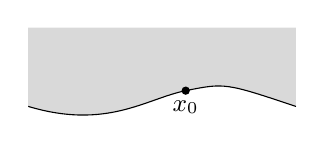
\begin{tikzpicture}
      \fill [gray, opacity=0.3] (0, 0) .. controls (1, -0.3) and (1.5, 0.1) .. (2, 0.2) .. controls (2.5, 0.3) .. (3.4, 0) -- (3.4, 1) -- (0, 1) -- cycle;
      \draw (0, 0) .. controls (1, -0.3) and (1.5, 0.1) .. (2, 0.2) .. controls (2.5, 0.3) .. (3.4, 0);

      \node [circ] at (2, 0.2) {};
      \node [below] at (2, 0.2) {\small$x_0$};
    \end{tikzpicture}
  \end{center}
  The idea is that given a $u$ defined on $U$, we can shift it downwards by some $\varepsilon$. It is a known result that translation is continuous, so this only changes $u$ by a tiny bit. We can then mollify with a $\bar{\varepsilon} < \varepsilon$, which would then give a function defined on $U$ (at least locally near $x_0$).

  So fix some $x_0 \in \partial U$. Since $\partial U$ is $C^{0, 1}$, there exists $r > 0$ such that $\gamma \in C^{0, 1}(\R^{n - 1})$ such that
  \[
    U \cap B_r(x_0) = \{(x', x_n) \in B_r(x') \mid x_n > \gamma(x')\}.
  \]
  Set
  \[
    V = U \cap B_{r/2}(x^0).
  \]
  Define the shifted function $u_\varepsilon$ to be
  \[
    u_\varepsilon(x) = u(x + \varepsilon e_n).
  \]
  Now pick $\bar{\varepsilon}$ sufficiently small such that
  \[
    v^{\varepsilon, \bar{\varepsilon}} = \eta_{\bar{\varepsilon}} * u_\varepsilon
  \]
  is well-defined. Note that here we need to use the fact that $\partial U$ is $C^{0, 1}$. Indeed, we can see that if the slope of $\partial U$ is very steep near a point $x$:
  \begin{center}
    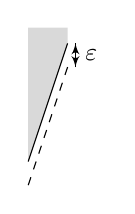
\begin{tikzpicture}
      \fill [gray, opacity=0.3] (0, 0) -- (0.5, 1.5) -- (0.5, 1.7) -- (0, 1.7);
      \draw (0, 0) -- (0.5, 1.5);

      \draw [dashed] (0, -0.3) -- (0.5, 1.2);

      \draw [-latex'] (0.6, 1.2) -- (0.6, 1.5) node [pos=0.5, right] {\small$\varepsilon$};
      \draw [latex'-] (0.6, 1.2) -- (0.6, 1.5);
    \end{tikzpicture}
  \end{center}
  then we need to choose a $\bar{\varepsilon}$ much smaller than $\varepsilon$. By requiring that $\gamma$ is $1$-H\"older continuous, we can ensure there is a single choice of $\bar{\varepsilon}$ that works throughout $V$. As long as $\bar{\varepsilon}$ is small enough, we know that $v^{\varepsilon, \bar{\varepsilon}} \in C^\infty(\bar{V})$.

  Fix $\delta > 0$. We can now estimate
  \begin{align*}
    \|v^{\varepsilon, \tilde{\varepsilon}} - u\|_{W^{k. p}(V)} &= \|v^{\varepsilon, \tilde{\varepsilon}} - u_\varepsilon + u_\varepsilon - u\|_{W^{k, p}(V)}\\
    &\leq \|v^{\varepsilon, \tilde{\varepsilon}} - u_\varepsilon\|_{W^{k, p}(V)} + \|u_\varepsilon - u\|_{W^{k. p}(V)}.
  \end{align*}
  Since translation is continuous in the $L^p$ norm for $p < \infty$, we can pick $\varepsilon > 0$ such that $\|u_\varepsilon - u\|_{W^{k. p}(V)} < \frac{\delta}{2}$. Having fixed such an $\varepsilon$, we can pick $\tilde{\varepsilon}$ so small that we also have $\|v^{\varepsilon, \tilde{\varepsilon}} - u_\varepsilon\|_{W^{k. p}(V)} < \frac{\delta}{2}$.

  The conclusion of this is that for any $x_0 \in \partial U$, we can find a neighbourhood $V \subseteq U$ of $x_0$ in $U$ such that for any $u \in W^{k, p}(U)$ and $\delta > 0$, there exists $v \in C^\infty(\bar{V})$ such that $\|u - v\|_{W^{k, p}(V)} \leq \delta$.

  It remains to patch all of these together using a partition of unity. By the compactness of $\partial U$, we can cover $\partial U$ by finitely many of these $V$, say $V_1, \ldots, V_N$. We further pick a $V_0$ such that $V_0 \Subset U$ and
  \[
    U = \bigcup_{i = 0}^N V_i.
  \]
  We can pick approximations $v_i \in C^\infty(\bar{V}_i)$ for $i = 0, \ldots, N$ (the $i = 0$ case is given by the previous global approximation theorem), satisfying $\|v_i - u\|_{W^{k, p}(V_i)} \leq \delta$.
%
%  Define the shifted point
%  \[
%    x^{\varepsilon} = x + \lambda\varepsilon e_n
%  \]
%  for $x \in V$, $\varepsilon > 0$.
%
%  For $\lambda > 0$ large enough and $\varepsilon$ sufficiently small, we have
%  \[
%    B_\varepsilon(x') \subseteq U \cap B_r(x^0).
%  \]
%  We can do this uniformly for all points $x \in V$ by the fact that $\gamma \in C^{0, 1}$.
%
%  We define $u_\varepsilon(x) = u(x^\varepsilon)$ for all $x \in V$. Set
%  \[
%    v^{\varepsilon, \tilde{\varepsilon}} = \eta_{\tilde{\varepsilon}} * u_\varepsilon
%  \]
%  for some $0 < \tilde{\varepsilon} < \varepsilon$. As a result, $v^{\varepsilon, \tilde{\varepsilon}} \in C^\infty(\bar{V})$.
%
%  Now fix $\delta > 0$. We estimate
%  \begin{align*}
%    \|v^{\varepsilon, \tilde{\varepsilon}} - u\|_{W^{k. p}}(V) &= \|v^{\varepsilon, \tilde{\varepsilon}} - u_\varepsilon + u_\varepsilon - u\|_{W^{k, p}(V)}\\
%    &\leq \|v^{\varepsilon, \tilde{\varepsilon}} - u_\varepsilon\|_{W^{k, p}(V)} + \|u_\varepsilon - u\|_{W^{k. p}(V)}.
%  \end{align*}
%  Since translation is continuous in the $L^p$-norms for $p < \infty$, we can pick $\varepsilon > 0$ such that $\|u_\varepsilon - u\|_{W^{k p}(V)} < \frac{\delta}{2}$.
%
%  Having fixed $\varepsilon$, we can then pick $\tilde{\varepsilon}$ so that $\|v^{\varepsilon, \tilde{\varepsilon}} - u_\varepsilon\|_{W^{k. p}(V)} < \frac{\delta}{\varepsilon}$.
%
%  Now since $\partial U$ is compact, we can cover $\partial U$ by finitely many of these $V$'s. More precisely, we can find finitely many $x_i^0 \in \partial U$, radii $r_i > 0$, sets $V_i = U \cap B_{r_i/2}(x_i^0)$ and functions $v_i \in C^\infty(\bar{V}_i)$ for $i = 1, \ldots, N$, such that
%  \[
%    \partial U \subseteq \bigcup_{i = 1}^N B_{r_i/2}(x_i^0).
%  \]
%  and
%  \[
%    \|v_i - u\|_{W^{k, p}(V_i)} \leq \delta.
%  \]
%  Finally, take an open $V_0 \Subset U$ such that
%  \[
%    C \subseteq \cup_{i = 0}^N V_i.
%  \]
%  By the previous theorem, we can choose $v_0 \in C^{\infty}(\bar{V}_0$ such that $\|v_0 - u\|_{W^{k, p}(V_0)} \leq \delta$.
%
  Pick a partition of unity $\{\zeta_i\}_{i = 0}^N$ of $\bar{U}$ subordinate to $\{V_i\}$. Define
  \[
    v = \sum_{i = 0}^N \zeta_i v_i.
  \]
  Clearly $v \in C^\infty(\bar{U})$, and we can bound
  \begin{align*}
    \|D^\alpha v - \D^\alpha u\|_{L^p(U)} &= \norm{\D^\alpha \sum_{i = 0}^N \zeta_i v_i - \D^\alpha \sum_{i = 0}^N \zeta_i u}_{L^p(U)}\\
    &\leq C_k \sum_{i = 0}^N \|v_i - u\|_{W^{k. p}(V_i)}\\
    &\leq C_k(1 + N)\delta,
  \end{align*}
  where $C_k$ is a constant that solely depends on the derivatives of the partition of unity, which are fixed. So we are done.
\end{proof}

\subsection{Extensions and traces}
\begin{thm}[Extension of $W^{1. p}$ functions]
  Suppose $U$ is open, bounded and $\partial U$ is $C^1$. Pick a bounded $V$ such that $U \Subset V$. Then there exists a bounded linear operator
  \[
    E: W^{1, p}(U) \to W^{1. p}(\R^n)
  \]
  for $1 \leq p < \infty$ such that for any $u \in W^{1, p}(U)$,
  \begin{enumerate}
    \item $Eu = u$ almost everywhere in $U$
    \item $Eu$ has support in $V$
    \item $\|Eu\|_{W^{1, p}(\R^n)} \leq C \|u\|_{W^{1, p}(U)}$, where the constant $C$ depends on $U, V, p$ but not $w$.
  \end{enumerate}
\end{thm}
We'll prove this later. First we need to look a bit more at $\partial U$. Since $\partial U$ is $C^1$, for any $p \in \partial U$, there exists $r > 0$ and $\gamma \in C^1(\R^{n - 1})$ such that
\[
  U \cap B_r(p) = \{(x', x^n) \in B_r(p) \mid x^n > \gamma(x')\}.
\]
It's often convenient to ``straighten out'' the boundary. We define a map $\Phi: \R^n \to \R^n$ by
\begin{align*}
  \Phi(x)^i &= x^i & i &= 1, \ldots, n -1\\
  \Phi(x)^n &= x_n - \gamma(x_1, \ldots, x_n)
\end{align*}
This is clearly invertible with inverse, say, $\Psi$. The key point is that
\[
  \Phi(U \cap B_r(p)) \subseteq \{y_n > 0\},
\]
and $\Phi, \Psi$ are both $C^1$ with $\det \D \Phi = \det \D \Psi = 1$.

In other words, $\Phi$ is a $C^1$ diffeomorphism.

\begin{proof}
  Fix some point $x^0 \in \partial U$ and suppose that $\partial U$ near $x^0$ lying in the plane $\{x_n = 0\}$. We may assume that there exists $r > 0$ such that
  \begin{align*}
    B_+ &= B_r(x^0) \cap \{x_n \geq 0\} \subseteq \bar{U}\\
    B_- &= B_r(x^0) \cap \{x_n \leq 0\} \subseteq \R^n \setminus U.
  \end{align*}
  Suppose temporarily that $u \in C^1(\bar{U})$. The idea is that we want to reflect $u|_{B_+}$ across the $x_n = 0$ boundary to get a function on $B_{-}$, but the derivative will not be continuous if we do this. So we define a ``higher order reflection'' by
  \[
    \bar{u}(x) =
    \begin{cases}
      u(x) & x \in B^+\\
      -3u(x', -x_n) + 4\left(u x', -\frac{x_n}{2}\right) & x \in B_-
    \end{cases}
  \]
  \begin{center}
    \begin{tikzpicture}
      \draw [->] (-3, 0) -- (3, 0) node [right] {$x^n$};
      \draw [->] (0, -3) -- (0, 3) node [above] {$u$};

      \draw [domain=-2.1:0, mblue, thick] plot (\x, {- 1/3 * \x^3});
      \draw [domain=0:1.55, mblue, thick, dashed] plot (\x, {-5/6 * \x^3});
      \node [circ] at (-0.75, 0.14) {};
      \node [circ] at (-1.5, 1.124) {};
      \node [circ] at (1.5, -2.815) {};

      \draw (-1.5, 1.124) -- (1.5, -2.815);

      \draw [dashed] (-1.5, 1.124) -- (-1.5, 0) node [below] {$-x$};
      \draw [dashed] (-0.75, 0.14) -- (-0.7, 0) node [below] {$-\frac{x}{2}$};

      \draw [dashed] (1.5, -2.815) -- (1.5, 0) node [anchor = north west] {$x$};
    \end{tikzpicture}
  \end{center}
  We see that this is a continuous function. Moreover, by explicitly computing the partial derivatives, we see that they are continuous across the boundary. So we know $\bar{u} \in C^1(B_r(x^0))$.

  We can then easily check that we have
  \[
    \|\bar{u}\|_{W^{1, p}(B_r(x^0))} \leq C \|u\|_{W^{1, p}(B_+)}
  \]
  for some constant $C$.

  If $\partial U$ is not necessarily flat near $x^0 \in \partial U$, then we can use a $C^1$ diffeomorphism to straighten it out (exercise!).


  Since $\partial U$ is compact, we can take a finite number of points $x_i^0 \in \partial W$, sets $W_i$ and extensions $U_i \in C^1(W_i)$ extending $u$ such that
  \[
    \partial U \subseteq \bigcup_{i = 1}^N W_i.
  \]
  Pick $W_0 \Subset U$ such that $U \subseteq \bigcup_{i = 0}^N W_i$.

  Let $\{\zeta_i\}_{i = 0}^N$ be a partition of unity subordinate to $\{W_i\}$. Write
  \[
    \bar{u} = \sum_{i = 0}^N \zeta_i \bar{u}_i
  \]
  where $\bar{u}_0 = u$. Then $\bar{u} \in C^1(\R^n)$, $\bar{u} = u$ on $U$, and we have
  \[
    \|\bar{u}\|_{W^{1, p}(\R^n)} \leq C \|u\|_{W^{1, p}(U)}.
  \]
  By multiplying $\bar{u}$ by a cut-off, we may assume $\supp \bar{u} \subseteq V$ for some $V \Supset U$.

  Now notice that the whole construction is linear in $u$. So we have constructed a bounded linear operator from a dense subset of $W^{1, p}(U)$ to $W^{1,p}(V)$, and there is a unique extension to the whole of $W^{1, p}(U)$ by the completeness of $W^{1, p}(V)$. We can see that the desired properties are preserved by this extension.
\end{proof}

\subsubsection*{Trace theorems}
Since $u \in W^{1, p}(U)$ is only defined up to sets of measure zero, and $\partial U$ is typically a set of measure zero, we can't naively define $u|_{\partial U}$. But if we want to talk about boundary value problems, then we need a reasonable way to talk about the restriction of $u$ to the boundary. This is given by the trace theorem.

\begin{thm}[Trace theorem]\index{trace theorem}
  Assume $U$ is bounded and has $C^1$ boundary. Then there exists a bounded linear operator $T: W^{1, p}(U) \to L^p(\partial U)$ for $1 \leq p < \infty$ such that $Tu = u|_{\partial U}$ if $u \in W^{1, p}(U) \cap C(\bar{U})$.
\end{thm}
We say $Tu$ is the \term{trace} of $u$.

\begin{proof}
  It suffices to show that the restriction map defined on $C^\infty$ functions is a bounded linear operator, and then we have a unique extension to $W^{1, p}(U)$. The gist of the argument is that Stokes' theorem allows us to express the integral of a function over the boundary as an integral over the whole of $U$. In fact, the proof is indeed just the proof of Stokes' theorem.

  By general partition of unity arguments, it suffices to show this in the case where $U = \{x_n > 0\}$ and $u \in C^\infty{\bar{U}}$ with $\supp u \subseteq B_R(0) \cap \bar{U}$. Then
  \[
    \int_{\R^{n - 1}} |u(x', 0)|^p \;\d x' = \int_{\R^{n - 1}} \int_0^\infty \frac{\partial}{\partial x_n} |u(x', x_n)|^p \;\d x_n \;\d x' = \int_U p |u|^{p - 1} \sgn u \;\d x_n x'.
  \]
  We estimate this using Young's inequality to get
  \[
    \int_{\R^{n - 1}} |u(x', 0)|^p \;\d x' \leq C_p \int_U |u|^p + |u_{x_n}|^p \;\d U \leq C_p \|u\|_{W^{1, p}(U)}^p.
  \]
  So we are done.
\end{proof}
We can apply this to each derivative to define trace maps $W^{k, p}(U) \to W^{k - 1, p}(U)$.

In general, this trace map is not surjective. So in some sense, we don't actually need to use up a whole unit of differentiability. In the example sheet, we see that in the case $p = 2$, we only lose ``half'' a derivative.

Note that $C_c^\infty(U)$ is dense in $W_0^{1, p}(U)$, and the trace vanishes on $C_c^\infty(U)$. So $T$ vanishes on $W_0^{1, p}(U)$. In fact, the converse is true --- if $Tu = 0$, then $u \in W_0^{1, p}(U)$.

\subsection{Sobolev inequalities}
These are a collection of inequalities that allow us to trade differentiability against integrability.

The basic result is the Gagliardo--Nirenberg--Sobolev inequality. Before we try to prove or even state this, we first prove a technical lemma.
\begin{lemma}
  Let $n \geq 2$ and $f_1, \ldots, f_n \in L^{n - 1}(\R^{n - 1})$. For $1 \leq i \leq n$, denote
  \[
    \tilde{x}_i = (x_1, \ldots, x_{i - 1}, x_{i + 1}, \ldots, x_n),
  \]
  and set
  \[
    f(x) = f_1(\tilde{x}_1) \cdots f_n(\tilde{x}_n).
  \]
  Then $f \in L^1(\R^n)$ with
  \[
    \|f\|_{L^1}(\R^n) \leq \prod_{i = 1}^n \|f_i\|_{L^{n - 1}(\R^{n - 1})}.
  \]
\end{lemma}

\begin{proof}
  We prove by induction on $n$.

  If $n = 2$, then this is easy, since
  \[
    f(x_1, x_2) = f_1(x_2) f_2(x_1).
  \]
  So
  \begin{align*}
    \int_{\R^2}|f(x_1, x_2)| \;\d x &= \int |f_1(x_2)|\;\d x_2 \int |f_2(x_1)\;\d x_1\\
    &= \|f_1\|_{L^1(\R^1)} \|f_2\|_{L^1(\R^1)}.
  \end{align*}
  Suppose that the result is true for $n \geq 2$, and consider the $n + 1$ case. Write
  \[
    f(x) = f_{n + 1}(\tilde{x_{n + 1}}) F(x),
  \]
  where $F(x) = f_1(\tilde{x}_1) \cdots f_n(\tilde{x}_n)$. Then by H\"older's inequality, we have
  \begin{multline*}
    \int_{x_1, \ldots, x_n} |f(\ph, x_{n + 1})|\;\d x \leq \|f_{n + 1}\|_{L^n(\R^n)} \cdot \|F(\ph, x_{n + 1})\|_{L^{n/(n - 1)}(\R^n)}.
  \end{multline*}
  We now use the induction hypothesis to
  \[
    f_1^{n/(n - 1)} (\ph, x_{n + 1}) f_2^{n/(n - 1)}(\ph, x_{n + 1}) \cdots f_n^{n/(n - 1)}(\ph, x_{n + 1}).
  \]
  So
  \begin{align*}
    \int_{x_1, \ldots, x_n} |f(\ph, x_{n + 1})|\;\d x &\leq \|f_{n + 1}\|_{L^n(\R^n)}\\
    &\left(\prod_{i = 1}^n \|f_i^{n/(n-1)} (\ph, x_n)\|_{L^{n - 1}(\R^{n - 1})}\right)^{(n-1)/n}\\
    &= \|f_{n + 1}\|_{L^n(\R^n)} \prod_{i = 1}^n \|f_i(\ph, x_m)\|_{L^n(\R^{n - 1})}.
  \end{align*}
  Now integrate over $x_{n + 1}$. We get
  \begin{align*}
    \|f\|_{L^1(\R^{n + 1})} &\leq \|f_{n + 1}\|_{L^n(\R^n)} \int_{x_{n + 1}}\prod_{i = 1}^n \|f_i(\ph, x_{n + 1})\|_{L^n(\R^{n - 1})}\;\d x_n.\\
    &\leq \|f_{n + 1}\|_{L^n(\R^{n + 1})} \prod_{i = 1}^n \left(\int_{x_{n + 1}} \|f_i(\ph, x_{n + 1})\|^n_{L^n(\R^{n - 1})} \;\d x_{n + 1}\right)^{1/n}\\
    &= \|f_{n + 1}\|_{L^n(\R^n)} \prod_{i = 1}^n \|f_i\|_{L^n(\R^n)},
  \end{align*}
  as desired.
\end{proof}

\begin{thm}[Gagliardo--Nirenberg--Sobolev inequality]\index{Gagliardo--Nirenberg--Sobolev inequality}
  Assume $n > p$. Then we have
  \[
    W^{1, p}(\R^n) \subseteq L^{p^*}(\R^n),
  \]
  where
  \[
    p^* = \frac{np}{n - p} > p,
  \]
  and there exists $c > 0$ depending on $n, p$ such that
  \[
    \|u\|_{L^{p^*}(\R^n)} \leq c\|u\|_{W^{1, p}(\R^n)}.
  \]
  In other words, $W^{1, p}(\R^n)$ is continuously embedded in $L^{p^*}(\R^n)$.
\end{thm}

\begin{proof}
  Assume $u \in C_c^\infty(\R^n)$, and consider $p = 1$. Since the support is compact,
  \[
    u(x) = \int_{-\infty}^{x_i} u_{x_i}(x_1 ,\ldots, x_{i - 1}, y_i, x_{i + 1}, \ldots, x_n)\;\d y_i.
  \]
  So we know that
  \[
    |u(x)| \leq \int_{-\infty}^\infty |\D u(x_1, \ldots, x_{i - 1}, y_i, x_{i + 1}, \ldots, x_n)|\;\d y_i \equiv f_i(\tilde{x}_i).
  \]
  Thus, applying this once in each direction, we obtain
  \[
    |u(x)|^{n/(n - 1)} \leq \prod_{i = 1}^n f_i(\tilde{x}_i)^{1/(n - 1)}.
  \]
  If we integrate and then use the lemma, we see that
  \[
    \left(\|u\|_{L^{n/(n - 1)}(\R^n)}\right)^{n/(n - 1)} \leq C \prod_{i = 1}^n \|f_i^{1/(n - 1)}\|_{L^{n - 1}(\R^{n - 1})} = \|\D u\|_{L^1(\R^n)}^{n/(n-1)}.
  \]
  So
  \[
    \|u\|_{L^{n/(n-1)}(\R^n)} \leq C \|\D u\|_{L^1(\R^n)}.
  \]
  Since $C^\infty_c(\R^n)$ is dense in $W^{1, 1}(\R^n)$, the result for $p = 1$ follows.

  Now suppose $p > 1$. We apply the $p = 1$ case to
  \[
    v = |u|^\gamma
  \]
  for some $\gamma > 1$, which we choose later. Then we have
  \[
    \D v = \gamma \sgn u \cdot |u|^{\gamma - 1} \D u.
  \]
  So
  \begin{align*}
    \left(\int_{\R^n} |u|^{\gamma n/(n-1)} \;\d x\right)^{(n - 1)/n} &\leq \gamma \int_{\R^n} |u|^{\gamma - 1}|\D u|\;\d x\\
    &\leq \gamma \left(\int_{\R^n} |u|^{(\gamma - 1) \frac{p}{p - 1}}\;\d x\right)^{\frac{p - 1}{p}} \left(\int_{\R^n} |\D u|^p \;\d x\right)^{1/p}.
  \end{align*}
  We choose $\gamma$ such that
  \[
    \frac{\gamma n}{n - 1} = \frac{(\gamma - 1)p}{p - 1}.
  \]
  So we should pick
  \[
    \gamma = \frac{p(n - 1)}{n - p} > 1.
  \]
  Then we have
  \[
    \frac{\gamma n}{n - 1} = \frac{np}{n - p} = p^*.
  \]
  So
  \[
    \left(\int_{\R^n} |u|^{p^*}\;\d x\right)^{\frac{n - 1}{n}} \leq \frac{p(n - 1)}{n - p}\left(\int_{\R^n} |u|^{p^*}\;\d x \right)^{\frac{p - 1}{p}} \|\D u\|_{L^p(\R^n)}.
  \]
  So
  \[
    \left(\int_{\R^n}|u|^{p^*}\;\d x\right)^{1/p^*} \leq \frac{p(n - 1)}{n - p} \|\D u\|_{L^p(\R^n)}.
  \]
  This argument is valid for $u \in C_c^\infty(\R^n)$, and by approximation, we can extend to $W^{1, p}(\R^n)$.
\end{proof}

We can deduce some corollaries of this result:
\begin{cor}
  Suppose $U \subseteq \R^n$ is open and bounded with $C^1$-boundary, and $1 \leq p < n$. Then if $p^* = \frac{np}{n - p}$, we have
  \[
    W^{1, p}(U) \subseteq L^{p^*}(U),
  \]
  and there exists $C = C(U, p, n)$ such that
  \[
    \|u\|_{L^{p^*}(U)} \leq C\|u\|_{W^{1, p}(U)}.
  \]
\end{cor}

\begin{proof}
  By the extension theorem, we can find $\bar{u} \in W^{1, p}(\R^n)$ with $\bar{u} = u$ almost everywhere on $U$ and
  \[
    \|\bar{u}\|_{W^{1, p}(\R^n)} \leq C \|u\|_{W^{1, p}(U)}.
  \]
  Then we have
  \[
    \|u\|_{L^{p^*}(U)} \leq \|\bar{u}\|_{L^{p^*}(\R^n)} \leq C \|\bar{u}\|_{W^{1, p}(\R^n)} \leq \tilde{C} \|u\|_{W^{1, p}(U)}.
  \]
\end{proof}

\begin{cor}
  Suppose $U$ is open and bounded, and suppose $u \in W^{1, p}_0(U)$. For some $1 \leq p < n$, then we have the estimates
  \[
    \|u\|_{L^q(U)} \leq C \|\D u\|_{L^p(U)}
  \]
  for any $q \in [1, p^*]$. In particular,
  \[
    \|u\|_{L^p(U)} \leq C \|\D u\|_{L^p(U)}.
  \]
\end{cor}

\begin{proof}
  Since $u \in W_0^{1, p}(U)$, there exists $u_0 \in C_c^\infty (U)$ converging to $u$ in $W^{1, p}(U)$. Extending $u_m$ to vanish on $U^c$, we have
  \[
    u_m \in C_c^\infty(\R^n).
  \]
  Applying Gagliardo--Nirenberg--Sobolev, we find that
  \[
    \|u_m\|_{L^{p^*}(\R^n)} \leq C \|\D u_m\|_{L^p(\R^n)}.
  \]
  So we know that
  \[
    \|u_m\|_{L^{p^*}(U)} \leq C \|\D u_m\|_{L^p(U)}.
  \]
  Sending $m \to \infty$, we obtain
  \[
    \|u\|_{L^{p^*}(U)} \leq C \|\D u\|_{L^p(U)}.
  \]
  Since $U$ is bounded, by H\"older, we have
  \[
    \left(\int_U |u|^q\;\d x\right)^{1/q} \leq \left(\int_U 1 \;\d x \right)^{1/rq} \left(\int_U |u|^{qs}\;\d s \right)^{1/sq} \leq C \|u\|_{L^{p^*}(U)}
  \]
  provided $q \leq p^*$, where we choose $s$ such that $qs = p^*$, and $r$ such that $\frac{1}{r} + \frac{1}{s} = 1$.
\end{proof}

Now suppose that $n < p < \infty$. We might hope that if $u \in W^{1, p}(\R^n)$, then $u$ is ``better than $L^\infty$''.

\begin{thm}[Morrey's inequality]\index{Morrey's inequality}
  Suppose $n < p < \infty$. Then there exists a constant $C$ depending only on $p$ and $n$ such that
  \[
    \|u\|_{C^{0, \gamma}(\R^n)} \leq C \|u\|_{W^{1, p}(\R^n)}
  \]
  for all $u \in C^\infty_c (\R^n)$ where $C = C(p, n)$ and $\gamma = 1 - \frac{n}{p} < 1$.
\end{thm}

\begin{proof}
  We first prove the H\"older part of the estimate.

  Let $Q$ be an open cube of side length $r > 0$ and containing $0$. Define
  \[
    \bar{u} = \frac{1}{|Q|} \int_Q u(x)\;\d x.
  \]
  Then
  \begin{align*}
    |\bar{u} - u(0)| &= \left|\frac{1}{|Q|} \int_Q [u(x) - u(0)]\;\d x\right|\\
    &\leq \frac{1}{|Q|} \int_Q |u(x) - u(0)|\;\d x.
  \end{align*}
  Note that
  \[
    u(x) - u(0) = \int_0^1 \frac{\d}{\d t} (u(t)x)\;\d t = \sum_i \int_0^1 x^i \frac{\partial u}{6 x^i} (tx)\;\d t.
  \]
  So
  \[
    |u(x) - u(0)| \leq r \int_0^1 \sum_i \left|\frac{\partial u}{\partial x^i} (tx)\right|\;\d t.
  \]
  So we have
  \begin{align*}
    |\bar{u} - u(0)| &\leq \frac{r}{|Q|} \int_Q \int_0^1 \sum_i \left|\frac{\partial u}{\partial x^i}(tx)\right|\;\d t\;\d x\\
    &= \frac{r}{|Q|} \int_0^1 tt^{-n} \left(\int_{tQ} \sum_i \left|\frac{\partial u}{\partial x^i} (y)\right|\;\d y \right)\;\d t\\
    &\leq \frac{r}{|Q|} \int_0^1 t^{-n} \left(\sum_{i = 1}^n \left\|\frac{\partial u}{\partial x^i}\right\|_{L^p(tQ)} |tQ|^{1/p'}\right)\;\d t.
  \end{align*}
  where $\frac{1}{p} + \frac{1}{p'} = 1$.

  Using that $|Q| = r^n$, we obtain
  \begin{align*}
    |\bar{u} - u(0)| &\leq c r^{1 -n + \frac{n}{p'}} \|\D u\|_{L^p(\R^n)} \int_0^1 t^{-n + \frac{n}{p'}} \;\d t\\
    &\leq \frac{c}{1 - n/p} r^{1 - n/p} \|\D u\|_{L^p(\R^n)}.
  \end{align*}
  Note that the right hand side is decreasing in $r$. So when we take $r$ to be very small, we see that $u(0)$ is close to the average value of $u$ around $0$.

  Indeed, suppose $x, y \in \R^n$ with $|x - y| = \frac{r}{2}$. Pick a box containing $x$ and $y$ of side length $r$. Applying the above result, shifted so that $x$, $y$ play the role of $0$, we can estimate
  \[
    |u(x) - u(y)| \leq |u(x) - \bar{u}| + |u(y) - \bar{u}| \leq \tilde{C} r^{1 - n/p} \|\D u\|_{L^p(\R^n)}.
  \]
  Since $r < \|x - y\|$, it follows that
  \[
    \frac{|u(x) - u(y)|}{|x - y|^{1 - n/p}} \leq C \cdot 2^{1 - n/p} \|\D u\|_{L^p(\R^n)}.
  \]
  So we conclude that $[u]_{C^{0, \gamma}(\R^n)} \leq C \|\D u\|_{L^p(\R^n)}$.

  Finally, to see that $u$ is bounded, any $x \in \R^n$ belongs to some cube $Q$ of side length $1$. So we have
  \[
    |u(x)| \leq |u(x) - \bar{u} + \bar{u}| \leq |\bar{u}| + C \|\D u\|_{L^p(\R^n)}.
  \]
  But also
  \[
    |\bar{u}| \leq \int_Q |u(x)|\;\d x \leq \|u\|_{L^p(\R^n)} \|1\|_{L^p(Q)} = \|u\|_{L^p(\R^n)}.
  \]
  So we are done.
\end{proof}

\begin{cor}
  Suppose $u \in W^{1, p}(U)$ for $U$ open, bounded with $C^1$ boundary. Then there exists $u^* \in C^{0, \gamma}(U)$ such that $u = u^*$ almost everywhere and $\|u^*\|_{C^{0, \gamma}(U)} \leq C\|u\|_{W^{1, p}(U)}$.
\end{cor}

By applying these results iteratively, we can establish higher order versions
\[
  W^{k, p} \subseteq L^q(U)
\]
with some appropriate $q$.

\section{Elliptic boundary value problems}
Let's motivate our study by describing an elliptic boundary value problem.
\begin{eg}
  Suppose $U \subseteq \R^n$ is a bounded open set with smooth boundary. Suppose $\partial U$ is a perfect conductor and $\rho: U \to \R$ is the charge density inside $U$. The electrostatic field $\phi$ satisfies
  \begin{align*}
    \Delta \phi &= \rho\\
    \phi |_{\partial } &= 0.
  \end{align*}
  This is an example of an elliptic boundary value problem. Note that we cannot tackle this with the Cauchy--Kovalevskaya theorem, since we don't even have enough boundary conditions, and also because we want an everywhere-defined solution.
\end{eg}


\subsection{Second-order elliptic boundary value problems}
Let's now move on and try to apply some of this theory to try and understand elliptic PDEs.

Let $U \subseteq \R^n$ be open and bounded with $C^1$ boundary, and for $u \in C^2(\bar{U})$, we define
\[
  Lu = - \sum_{i, j = 1}^n (a^{ij}(x) u_j)_{x_i} + \sum_{i = 1}^n b^i(x) u_{x_i} + c(x) u,
\]
where $a^{ij}$, $b^i$ and $c$ are given functions defined on $U$. Typically, we will assume they are at least $L^\infty$, but sometimes we will require more.

If $a^{ij} \in C^1(U)$, then we can rewrite this as
\[
  Lu = - \sum_{i, j = 1}^n a^{ij}(x) u_{x_i x_j} + \sum_{i = 1}^n \tilde{b}^i(x) u_{x_i} + c(x) u
\]
for some $\tilde{b}^i$, using the product rule.

We will mostly use the first form, called the \term{divergence form}, which is suitable for the \emph{energy method}, while the second (non-divergence form) is suited to the maximum principle.

We further assume that $L$ is elliptic, i.e.
\[
  \sum_{i, j} a^{ij}(x) \xi_i \xi_j \geq 0
\]
for all $x \in U$ and $\xi \in \R^n$.

It turns out this is not quite strong enough, because this condition allows the $a_{ij}$'s to be degenerate, or vanish at the boundary.

\begin{defi}[Uniform ellipticity]\index{uniform ellipticity}
  An operator
  \[
    Lu = - \sum_{i, j = 1}^n (a^{ij}(x) u_j)_{x_i} + \sum_{i = 1}^n b^i(x) u_{x_i} + c(x) u
  \]
  is \emph{uniformly elliptic} if
  \[
    \sum_{i, j = 1}^n a^{ij}(x) \xi_i \xi_j \geq \theta |\xi|^2
  \]
  for some $\theta > 0$ and all $x \in U, \xi \in\R^n$.
\end{defi}

We shall consider the \term{boundary value problem}
\begin{align*}
  Lu &= f & \text{on }U\\
  u|_{\partial U} &= 0.
\end{align*}
This form of the equation is not very amenable to study by functional analytic methods. Let's suppose $u \in C^2(\bar{U})$ is a solution, and suppose $v \in C^2(\bar{U})$ also satisfies $v|_{\partial U} = 0$. Multiply the equation $Lu = f$ by $v$ and integrate by parts. Then we get
\[
  \int_U vf \;\d x = \int_U \left(\sum_{ij} v_{x_i} a^{ij} u_{x_j} + \sum_i b^i u_{x_i} + c u\right)\;\d x \equiv B[u, v].\tag{$(2)$}
\]
Conversely, suppose $u \in C^2(\bar{U})$ and $u|_{\partial U} = 0$. If $\int_U vf\;\d x = B[u, v]$ for all $v \in C^2(\bar{U})$ such that $v|_{\partial U} = 0$, then we claim $u$ in fact solves the original equation.

Indeed, undoing the integration by parts, we conclude that
\[
  \int v Lu \;\d x = \int v f\;\d x
\]
for all $v \in C^2(\bar{U})$ with $v|_{\partial U} = 0$. But if this is true for all $v$, then it must be that $Lu = f$.

Thus, the PDE problem we started with is equivalent to finding $u$ that solves $B[u, v] \int_U v f\;\d x$ for all suitable $v$, provided $u$ is regular enough.

On the other hand, $(2)$ makes sense for $u, v \in H_0^1(U)$. This motivates the following definition:

\begin{defi}[Weak solution]\index{weak solution}
  We say $u \in H_0^1(U)$ is a \emph{weak solution} of
  \begin{align*}
    Lu &= f & \text{on }U\\
    u|_{\partial U} &= 0
  \end{align*}
  for $f \in L^2(U)$ if
  \[
    B[u, v] = (f, v)_{L^2(U)}
  \]
  for all $v \in H_0^1(U)$.
\end{defi}

We'll exploit the Hilbert space structure of $H_0^1(U)$ to find weak solutions.

\begin{thm}[Lax--Milgram theorem]\index{Lax--Milgram theorem}
  Let $H$ be a real Hilbert space with inner product $(\ph, \ph)$. Suppose $B: H \times H \to \R$ is a bilinear mapping such that there exists constants $\alpha, \beta > 0$ so that
  \begin{itemize}
    \item $|B[u, v]| \leq \alpha \|u\| \|v\|$ for all $u, v \in H$ \hfill (boundedness)
    \item $\beta\|u\|^2 \leq B[u, u]$ \hfill (coercivity)
  \end{itemize}
  Then if $f: H \to \R$ is a bounded linear map, then there exists a unique $u \in H$ such that
  \[
    B[u, v] = \bra f, v\ket
  \]
  for all $v \in H$.
\end{thm}
Note that if $B$ is just the inner product, then this is the Riesz representation theorem.

\begin{proof}
  For each fixed $u \in H$, the map
  \[
    v \mapsto B[u, v]
  \]
  is a bounded linear functional on $H$. So by the Riesz representation theorem, we can find some $w$ such that $B[u, v] = (w, v)$. We write $w = Au$, so that
  \[
    B[u, v] = (Au, v).
  \]
  Since $B$ is bilinear, it is immediate that $A: H \to H$ is linear. Further,
  \[
    \|Au\|^2 = (Au, Au) = B[u, Au]\leq \alpha \|u\| \|Au\|.
  \]
  So $\|Au\| \leq \alpha \|u\|$. So $Au$ is bounded.

  Next, we assert that $A$ is injective, and has closed image. By coercivity, we know
  \[
    \beta \|u\|^2 \leq B[u, u] = (Au, u) \leq \|A u\| \|u\|.
  \]
  So it follows that
  \[
    \|u\| \leq \frac{1}{\beta} \|Au\|.
  \]
  So $A$ is bounded below, hence is injective and has closed image, since $H$ is complete. Indeed, injectivity is clear, and if $A u_m \to v$ for some $v$, then $\|u_m - u_n\| \leq \frac{1}{\beta} \|A u_m - A u_n\| \to 0$ as $m, n \to \infty$. So $(u_n)$ is Cauchy, and hence has a limit $u$. Then by continuity, $A u = v$, and in particular, $v \in \im A$.

  Since $\im A$ is closed, we know
  \[
    H = \im A \oplus \im A ^\perp.
  \]
  Now let $w \in \im A^\perp$. Then we can estimate
  \[
    \beta\|w\|^2 \leq B[w, w] = (Aw, w) = 0.
  \]
  So $w = 0$. Thus, in fact $\im A^\perp = \{0\}$, and so $A$ is surjective. By the inverse mapping theorem (or by a direct argument), $A^{-1}$ exists and is bounded linear. Now consider
  \[
    B[u, v] = \bra f, v\ket.
  \]
  By the Riesz representation theorem again, there is a unique $w \in H$ such that $\bra f, v\ket = (u, v)$. We can then set $u = A^{-1}w$. So
  \[
    B[u, v] = (Au, v) = (w, v) = \bra f, v\ket.
  \]
  To show uniqueness, suppose $u, \tilde{u}$ both satisfy $B[u, v] = \bra f, v\ket$. Then
  \[
    B[u - \tilde{u}, v] = 0.
  \]
  Taking $v = u - \tilde{u}$, this implies $u - \tilde{u} = 0$.
\end{proof}

We would like to apply this to our elliptic PDE. To do so, we need to prove that our $B$ satisfy boundedness and coercivity.

\begin{thm}[Energy estimates for $B$]\index{energy estimate}
  Suppose $a^{ij} = a^{ji}, b^i, c \in L^\infty(U)$, and there exists $\theta > 0$ such that
  \[
    \sum_{i, j = 1}^n a^{ij}(x) \xi_i \xi_j \geq \theta |\xi|2
  \]
  for almost every $x \in U$ and $\xi \in \R^n$. Then if $B$ is defined by
  \[
    B[u, v] = \int_U \left(\sum_{ij} v_{x_i} a^{ij} u_{x_j} + \sum_i b^i u_{x_i} + c u\right)\;\d x,
  \]
  then there exists $\alpha, \beta > 0$ and $\gamma \geq 0$ such that
  \begin{enumerate}
    \item $|B[u, v]| \leq \alpha \|u\|_{H^1(U)} \|v\|_{H^1(U)}$ for all $u, v \in H_0^1(U)$
    \item $\beta\|u\|^2_{H^1(U)} \leq B[u, u] + \gamma \|u\|_{L^2(U)}^2$.
  \end{enumerate}
\end{thm}

\begin{proof}\leavevmode
  \begin{enumerate}
    \item We estimate
      \begin{align*}
        |B[u, v]| &\leq \sum_{I, j} \|a^{ij}\|_{L^\infty(U)} \int_U |\D u| |\D v|\;\d x\\
        &\hphantom{{ {}={}}}+ \sum_i \|b\|_{C^\infty(U)} \int_U |\D u| |v| \;\d x\\
        &\hphantom{{ {}={}}}+ \|c\|_{L^\infty(U)} \int_U |u| |v| \;\d x\\
        &\leq c_1 \|\D u\|_{L^2(U)} \|\D v\|_{L^2(u)} + c_2 \| \D u\|_{L^2(U)} \|v\|_{L^2(U)} \\
        &+ c_3 \|u\|_{L^2(U)} \|v\|_{L^2(u)}\\
        &\leq \alpha \|u\|_{H^1(U)} \|v\|_{H^1(U)}
      \end{align*}
      for some $\alpha$.
    \item We start from uniform ellipticity. This implies
      \begin{align*}
        \theta \int_U |\D u|^2 \;\d x &\leq \int_U \sum_{i, j = 1}^n a^{ij}(x) u_{x_i} u_{x_j} \;\d x\\
        &= B[u ,u] - \int_U \sum_{i = 1}^n b^i u_{x_i} u + cu^2\;\d x\\
        &\leq B[u, u] + \sum_{i = 1}^n \|b^i\|_{L^\infty(U)} \int |\D u| |u| \;\d x + \|c\|_{L^\infty(U)} \int_U |u|^2\;\d x
      \end{align*}
      Now by Young's inequality, we have
      \[
        \int_U |\D u| |u| \;\d x \leq \varepsilon \int_U |\D u|^2 \;\d x + \frac{1}{4\varepsilon}\int_U |u|^2 \;\d x
      \]
      for any $\varepsilon > 0$. We choose $\varepsilon$ small enoguh so that
      \[
        \varepsilon\sum_{i = 1}^n \|b^i\|_{L^\infty(U)} \leq \frac{\theta}{2}.
      \]
      So we have
      \[
        \theta \int_U |\D u|^2 \;\d x \leq B[u, u] + \frac{\theta}{2} \int_U |\D u|^2 \;\d x + \gamma \int_U |u|^2\;\d x
      \]
      for some $\gamma$. This implies
      \[
        \frac{\theta}{2} \| \D u\|_{L^2(U)}^2 \leq B[u, u] + \gamma \|u\|_{L^2(U)}^2
      \]
      We can add $\frac{\theta}{2}\|u\|_{L^2(U)}^2$ on both sidesto get the desired bound on $\|u\|_{H^1(U)}$.
  \end{enumerate}
\end{proof}
Note that if $B$ corresponds to an operator with $b^i \equiv 0$ and $c \geq 0$, then we immediately have
\[
  \theta \int |\D u|^2 \;\d x \leq B[u, u].
\]
Recalling \term{Poincar\'e's inequality}: there is some $C > 0$ such that for all $u \in H_0^1 (U)$, we have
\[
  \|u\|_{L^2(U)} \leq C \|\D u\|_{L^2(U)}.
\]
Thus, we can take $\gamma = 0$.

The estimate (ii) is sometimes called \term{Grading's inequality}. % insert circle above a.

\begin{thm}
  Let $U, L$ be as above. There is a $\gamma \geq 0$ such that for any $\mu \geq \gamma$ and any $f \in L^2(U)$, there exists a unique weak solution to
  \begin{align*}
    Lu + \mu u &= f & \text{in $U$}\\
    u &= 0 & \text{on $\partial U$}.
  \end{align*}
  Moreover, we have
  \[
    \|u\|_{H^1(U)} \leq C \|f\|_{L^2(U)}
  \]
  for some $C = C(L, U) \geq 0$.
\end{thm}

\begin{proof}
  Take $\gamma$ from the previous theorem when applied to $L$. Then if $\mu \geq \gamma$ and we set
  \[
    B_\mu[u, v] = B[u, v] + \mu (u, v)_{L^2(U)},
  \]
  This i s the bilinear form corresponding to the operator
  \[
    L_\mu = L + \mu.
  \]
  Then by the previous theorem, $B_\mu$ satisfies boundedness and coercivity. So if we fix any $f \in L^2$, and think of it as an element of $H_0^1(U)^*$ by
  \[
    \bra f, v \ket = (f, u)_{L^2(U)} = \int_U fv\;\d x,
  \]
  then we can apply Lax--Milgram to find a unique $u \in H_0^1(U)$ satisfying $B_\mu[u, v] = \bra f, v\ket = (f, v)_{L^2(U)}$ for all $v \in H_0^1(U)$. This is precisely the condition for $u$ to be a weak solution.

  Finally, the Garding inequality tells us
  \[
    \beta \|u\|_{H^1(U)}^2 \leq B_\mu[u, u] = (f, u)_{L^2(U)} \leq \|f\|_{L^2(U)} \|u\|_{L^2(U)}.
  \]
  So we know that
  \[
    \beta \|u\|_{H^1(U)} \leq \|f\|_{L^2(U)}.
  \]
\end{proof}
In some way, this is a magical result. We managed to solve a PDE without having to actually work with a PDE. There are a few things we might object to. First of all, we only obtained a weak solution, and not a genuine solution. We will show that under some reasonable assumptions on $a, b, c$, if $f$ is better behaved, then $u$ is also better behaved, and in general, if $f \in H^k$, then $u \in H^{k + 2}$. This is known as \emph{elliptic regularity}. Together Sobolev inequalities, this tells us $u$ is genuinely a classical solution.

Another problem is the presence of the annoying $\mu$. We noted that if $L$ is, say, Laplace's equation, then we can take $\gamma = 0$, and so we don't have this problem. But in general, this theorem requires it, and this is a bit unsatisfactory. To fix this, we will look at compactness.

In the study of PDEs, compactness plays an important role. The basic result to keep in mind is the Bolzano--Weierstrass theorem, which says the following:
\begin{thm}[Bolzano--Weierstrass]\index{Bolzano--Weierstrass theorem}
  If $(x_n)_{n = 0}^\infty$ is a sequence of real numbers satisfying $|x_n| \leq K$ for all $n$ (and any fixed $K$), then $(x_n)$ admits a subsequence $(x_{n_i})_{i = 1}^\infty$ which converges to some $x$ with $|x| \leq K$.
\end{thm}

We would like a similar result for Hilbert spaces. Unfortunately, it is not true unless our Hilbert space is finite-dimensional. However, it turns out we can make analogous statement if we use a weaker version of convergence.

\begin{defi}[Weak convergence]\index{weak convergence}
  Suppose $(u_n)_{n = 1}^\infty$ is a sequence of $u_n \in H$ for $H$ a Hilbert space. We say $u_n$ \emph{converges weakly} to $u \in H$ if
  \[
    (u_n, w) \to (u, w)
  \]
  for all $w \in H$. We write $u_n \rightharpoonup u$.
\end{defi}

\begin{lemma}
  Weak limits are unique.\qedsym
\end{lemma}

\begin{lemma}
  Strong convergence implies weak convergence.\qedsym
\end{lemma}

\begin{thm}[Weak compactness]\index{weak compactness theorem}
  Let $H$ be a separable Hilbert space, and suppose $(u_m)_{m = 1}^\infty$ is a sequence with $u_m \in H$ sch that $\|u_m\| \leq K$ for all $m$. Then $u_m$ admits a subsequence $u_{m_j}$ such that $u_{m_j} \rightharpoonup u$ for some $u\ in H$, $\|u\| \leq K$.
\end{thm}

\begin{proof}
  Let $(e_i)_{i = 1}^\infty$ be an orthonormal basis for $H$. Consider $(e_1, u_m)$. By Cauchy--Schwarz, we have
  \[
    |(e_1, u_m)| \leq \|e_1\| \|e_m\| \leq K.
  \]
  So by Bolzano--Weierstrass, there exists a subsequence $(u_{m_j})$ such that $(e_1, u_{m_j})$ converges.

  Doing this iteratively, we can find a subsequence $(v_\ell)$ such that $(e_i, v_\ell) \to c_i$ as $j \to \infty$ for some $|c_i| \leq K$, for each $i$.

  We would expect the weak limit to be $\sum c_i e_i$. To prove this, we need to first show it converges. We have
  \begin{align*}
    \sum_{j = 1}^p |c_j|^2 &= \lim_{k \to \infty} \sum_{j = 1}^p |(e_j, v_\ell)|^2\\
    &\leq \sup \sum_{j = 1}^p |(e_j, v_\ell)|^2\\
    &\leq \sup \|v_k\|^2\\
    &\leq K^2,
  \end{align*}
  using Bessel's inequality. So
  \[
    u = \sum_{j = 1}^\infty c_j e_j
  \]
  converges in $H$, and $\|u\| \leq K$. We already have
  \[
    (e_j, v_{\ell}) \to (e_j, u)
  \]
  for all $j$.

  For a general $w$, we write
  \[
    w = \sum_{i = 1}^p (e_j, w) e_j + w_p,,
  \]
  with $w_p \to 0$ in $H$ as $p \to \infty$. Then
  \[
    |(w, v_\ell) - (w, u)| \leq |(w - w_p, v_\ell - v)| + |(w_p, v_\ell - u)|
  \]
  We can bound the second term by
  \[
    |(w_p, v_\ell - u)| \leq \|w_p\| \|v_\ell - u\| \leq 2K \|w_p\| \to 0.
  \]
  Given $\varepsilon > 0$, pick $p$ large enough such that $|(w_p, v_\ell - u)| < \frac{\varepsilon}{2}$. Now $w - w_p$ is a finite linear combination of the $e_j$'s, we can pick $\ell$ such that $|(w - w_p, v_\ell - u)| < \frac{\varepsilon}{2}$.
\end{proof}

\begin{lemma}[Poincar\'e revisited]
  Suppose $u \in H^1(\R^n)$. Let $Q = [\xi_1, \xi_1 + L] \times \cdots \times [\xi_n , \xi_n + L]$ be a cube of length $L$. Then we have
  \[
    \|u\|_{L^2(Q)}^2 \leq \frac{1}{|Q|} \left(\int_Q u(x) \;\d x\right)^2 + \frac{nL^2}{2} \|\D u\|_{L^2(Q)}^2.
  \]
\end{lemma}

\begin{proof}
  By approximation, we can assume $u \in C^\infty(\bar{Q})$. For $x,y \in Q$, we write
  \begin{align*}
    u(x) - u(y) &= \int_{y_1}^{x_1} \frac{\d}{\d t} u(t, x_1, \ldots, x_n)\;\d t\\
    &\hphantom{{}={}} + \int_{y_2}^{x_2} \frac{\d}{\d t} u(y_1, t, x_3, \ldots, x_n)\;\d t\\
    &\hphantom{{}={}} + \cdots\\
    &\hphantom{{}={}} + \int_{y_n}^{x_n} \frac{\d}{\d t} u(y_1, \ldots, y_{n - 1}, t)\;\d t.
  \end{align*}
  Squaring, we find that 
  \begin{align*}
    u(x)^2 + u(y)^2 - 2u(x) u(y) &= n\left(\int_{y_1}^{x_1} \frac{\d}{\d t} u(t, x_1, \ldots, x_n)\;\d t\right)^2\\
    &\hphantom{{}={}} + \cdots\\
    &\hphantom{{}={}} + n\left(\int_{y_n}^{x_n} \frac{\d}{\d t} u(y_1, \ldots, y_{n - 1}, t)\;\d t\right)^2.
  \end{align*}
  Now integrate over $x$ and $y$. On the left, we get
  \[
    \iint_{Q \times Q}\d x\;\d y (u(x)^2 + u(y)^2 - 2u(x) u(y)) = 2 |Q| \|u\|_{L^2(Q)}^2 - 2 \left(\int_Q u(x) \;\d x\right)^2.
  \]
  On the right we have
  \begin{align*}
    I_1 &= \left(\int_{y_1}^{x_1} \frac{\d}{\d t} u(t, x_2, \ldots, x_n)^2 \;\d t\right)^2\\
    &\leq \int_{y_1}^{x_1} \;\d t \int_{y_1}^{x_1}\left(\frac{\d}{\d t} u(t, x_2, \ldots, x_n)\right)^2 \;\d t\\
    &\leq L \int_{\xi_1}^{\xi_1 + L} \left(\frac{\d}{\d t} u(t, x_2, \ldots, x_n)\right)^2 \;\d t.
  \end{align*}
  Integrating over all $x, y \in Q$, we get
  \[
    \iint_{Q \times Q}\d x\;\d y\; I_1 \leq L^2 |Q| \|\D_1 u\|_{L^2(Q)}^2.
  \]
  Similarly estimating the terms on the right-hand side, we find that
  \[
    2|Q| \|u\|_{L^2(Q)} - 2 \left(\int_Q u(x)\;\d x\right)^2 \leq n |Q| \sum_{i = 1}^n \|\D _i u\|^2_{L^2(Q)} = n |Q| L^2 \|\D u\|^2_{L^2(Q)}.
  \]
\end{proof}
With this estimate, we are now ready to prove
\begin{thm}[Rellich--Kondrachov]\index{Rellich--Kondrachov theorem}
  Suppose $U \subseteq \R^n$ is open, bounded with $C^1$ boundary. Let $(u_m)_{m = 1}^\infty$ be a sequence $u_m \in H^1(U)$ and $\|u_m\|_{H^1(U)} \leq K$. Then there exists $u \in H^1(U)$ and a subsequence $(u_m)_{m = 0}^\infty$ with $u_{m_j} \rightharpoonup u$ in $H^1(U)$ and $u_{m_j} \to u$ in $L^2(U)$.
\end{thm}

\begin{proof}
  By the extension theorem, we may assume $u_m \in H^1_0(Q)$ for some large cube $Q$ with $U \Subset Q$.

  By weak compactness, there exists $u \in H_0^1(Q)$ and a subsequence $u_{m_j}$ such that $u_{m_j} \rightharpoonup u$.

  Set $\omega_j = u_{m_j}$. We need to show that
  \[
    \|\omega_j - u\|_{L^2(Q)} \to 0.
  \]
  Fix $\delta > 0$. We can then cover $Q$ exactly by some number $k(\delta)$ cubes of side length $L < \delta$, such that the cubes intersect only at their faces. Call these $\{Q_a\}_{a = 1}^{k(\delta)}$.

  We apply Poincar\'e separately to each of these. Then we have
  \begin{align*}
    \|\omega_j - u\|_{L^2(Q)}^2 &= \sum_{a = 1}^{k(\delta)} \|\omega_j - u\|_{L^2(Q_a)}^2\\
    &\leq \sum_{a = 1}^{k(\delta)} \left[\frac{1}{|Q_a|} \left(\int_{Q_a} \omega_i - u\;\d x\right)^2 + \frac{n^2 \delta^2}{2} \|\D \omega_i - \D u\|^2_{L^2(Q_a)}\right]\\
    &= \sum_{a = 1}^{k(\delta)} \frac{1}{|Q_a|} \left(\int_{Q_a} \omega_i - u\;\d x\right)^2 + \frac{n^2 \delta^2}{2} \|\D \omega_i - \D u\|^2_{L^2(Q_a)}.
  \end{align*}
  Now we know $\|\D \omega_j - \D u\|_{L^2(Q)}^2 \leq \tilde{K}$ for some $\tilde{K}$. So for $\delta$ small enough, we may assume the second term is $< \frac{\varepsilon}{2}$.

  By the convergence $\omega_j \rightharpoonup u$, we have
  \[
    \int_{Q_1} u_j - u\;\d x \to 0
  \]
  for all $a$, since this is just the inner product with the constant function $1$. So for $i$ large enough, we have
  \[
    \frac{1}{|Q_a|} \left(\int_{Q_a} w_j - u \;\d x\right)^2 < \frac{\varepsilon}{2}.
  \]
\end{proof}
\printindex
\end{document}
